\documentclass[master, och, coursework]{SCWorks}
% Тип обучения (одно из значений):
%    bachelor   - бакалавриат (по умолчанию)
%    spec       - специальность
%    master     - магистратура
% Форма обучения (одно из значений):
%    och        - очное (по умолчанию)
%    zaoch      - заочное
% Тип работы (одно из значений):
%    coursework - курсовая работа (по умолчанию)
%    referat    - реферат
%    otchet     - универсальный отчет
%    nirjournal - журнал НИР
%    diploma    - дипломная работа
%    pract      - отчет о научно-исследовательской работе
%    autoref    - автореферат выпускной работы
%    assignment - задание на выпускную квалификационную работу
%    review     - отзыв руководителя
%    critique   - рецензия на выпускную работу
% Включение шрифта
%    times      - включение шрифта Times New Roman (если установлен)
%                 по умолчанию выключен
\usepackage{preamble}

\begin{document}

% Кафедра (в родительном падеже)
\chair{Информатики и программирования}

% Тема работы
\title{Разработка платформы единого резюме}

% Курс
\course{1}

% Группа
\group{173}

% Факультет (в родительном падеже) (по умолчанию "факультета КНиИТ")
% \department{факультета КНиИТ}

% Специальность/направление код - наименование
% \napravlenie{02.03.02 "--- Фундаментальная информатика и информационные технологии}
\napravlenie{02.04.03 "--- Математическое обеспечение и администрирование информационных систем}
% \napravlenie{09.03.01 "--- Информатика и вычислительная техника}
% \napravlenie{09.03.04 "--- Программная инженерия}
% \napravlenie{10.05.01 "--- Компьютерная безопасность}

% Для студентки. Для работы студента следующая команда не нужна.
% \studenttitle{Студентки}

% Фамилия, имя, отчество в родительном падеже
\author{Кулакова Максима Сергеевича}

% Руководитель НИР
\nirtitle{к.\,э.\,н., доцент} % степень, звание
\nirname{Л.\,В.\,Кабанова}

% Заведующий кафедрой
\chtitle{к.\,ф.-м.\,н.} % степень, звание
\chname{М.\,В.\,Огнева}

% Научный руководитель (для реферата преподаватель проверяющий работу)
\satitle{к.\,э.\,н., доцент} %должность, степень, звание
\saname{Л.\,В.\,Кабанова}

% Руководитель практики от организации (только для практики, для остальных типов
% работ не используется)
\patitle{к.\,э.\,н., доцент}
\paname{Л.\,В.\,Кабанова}

% Семестр (только для практики, для остальных типов работ не используется)
\term{1}

% Наименование практики (только для практики, для остальных типов работ не
% используется)
\practtype{производственная распределенная (научно-исследовательская работа)}

% Продолжительность практики (количество недель) (только для практики, для
% остальных типов работ не используется)
\duration{18}

% Даты начала и окончания практики (только для практики, для остальных типов
% работ не используется)
\practStart{01.09.2022}
\practFinish{15.01.2023}

% Год выполнения отчета
\date{2023}

\maketitle

% Включение нумерации рисунков, формул и таблиц по разделам (по умолчанию -
% нумерация сквозная) (допускается оба вида нумерации)
\secNumbering

\tableofcontents

% Раздел "Обозначения и сокращения". Может отсутствовать в работе
% \abbreviations
% \begin{description}
%     \item ... "--- ...
%     \item ... "--- ...
% \end{description}

% Раздел "Определения". Может отсутствовать в работе
% \definitions

% Раздел "Определения, обозначения и сокращения". Может отсутствовать в работе.
% Если присутствует, то заменяет собой разделы "Обозначения и сокращения" и
% "Определения"
% \defabbr

% Ссылка на источник в тексте
% \cite{}

\intro
Вопрос поиска работы всегда находился перед лицом человека, ведь работа должна 
приносить не только деньги, но и удовлетворение физических и психологических 
потребностей человека. Наиболее актуальной проблемой со стороны соискателя является 
то, где искать необходимого ему работодателя, а также с какой стороны преподнести 
свои навыки и умения, чтобы в ближайшие дни занимать рабочее место своей мечты.

В настоящее время для поиска работы в интернете существует множество сервисов, 
при помощи которых работодатели могут как выкладывать свои вакансии, так и 
рассматривать входящие предложения от соискателей. Некоторые из платформ для 
поиска работы предоставляют возможность создавать резюме напрямую в личном 
кабинете соискателя.

Из-за того, что существует огромное количество сервисов для поиска работы, 
кому-то из работодателей не всегда будет удобна та или иная платформа, 
и своё предпочтение он отдаст “третьей”. Соискателю становится труднее 
ориентироваться в сайтах для поиска нужной вакансии, особенно если резюме 
на них висит уже долгое время, а навыки человека успели обновиться, что 
требует уже его дальнейшее обновление. Держать под контролем несколько 
резюме на нескольких сайтах становится всё сложнее,что становится проблемой 
для активного соискателя.

Целью научно-исследовательской работы является разработка платформы единого 
резюме с привязкой и последующим его обновлением на различных сервисах 
поиска работы (таких как GitHub, Хабр Карьера, hh.ru).

Задачами работы являются следующие пункты:
\begin{enumerate}
    \item Обзор научной литературы (в том числе научно-технической) по теме 
    <<Разработка платформы единого резюме>>;
    \item Рассмотрение и анализ существующих платформ для создания резюме;
    \item Формулировка собственных методов разработки единой платформы резюме;
    \item Реализация клиентской и серверной частей платформы;
    \item Подведение итогов проведенной научно-исследовательской работы.
\end{enumerate}


% После введения — серии \section, \subsection и т.д.
\newpage
\section{Анализ научной литературы}
Рассматриваемая литература будет затрагивать тему аспектов составления резюме, 
принципы их составления и критерии, по которым работодателю с наибольшей вероятностью 
понравится грамотно составленное резюме. После проведения анализа данной темы нам 
предоставится возможность выделить основные пункты, которые будут учитываться 
при разработке собственной единой платформе резюме.

Для начала стоит рассмотреть научные статьи, связанные с доказательством важности 
правильного составления резюме в настоящее время, и какие изменения  оно претерпевает. 
В статье К.В. Косолаповой <<Типологические особенности современного резюме на английском 
языке>> автор выделяет основные пункты в резюме, которые было принято считать достаточными:
\begin{enumerate}
    \item Полные ФИО;
    \item Возраст;
    \item Место проживания на текущий момент;
    \item Место учёбы, уровень образования;
    \item Список умений;
    \item Опыт работы (при его наличии);
    \item Контактные данные.
\end{enumerate}

Автор также подчёркивает, что резюме является <<визитной карточкой>> для работодателя, 
и в зависимости от того, как оно составлено, будет зависеть решение
о приглашении соискателя на собеседование. В статье раскрывается современное 
понятие <<резюме>>, а также отмечается, что постепенное развитие и становление 
резюме определило его типологическое разнообразие. Так, традиционными типами 
резюме принято считать хронологическое (Chronological CV), функциональное 
(Functional CV) и комбинированное (Combination CV). После обзора 
на каждый из типов резюме автор рекомендует придерживаться следующим пунктам при 
составлении документа:
\begin{enumerate}
    \item Личные сведения в начале резюме (имя, адрес, контактные телефоны, 
    адрес электронной почты); 
    \item Краткое описание себя от первого или третьего лица в виде небольшого параграфа;
    \item Список ключевых навыков, умений соискателя, а также занимаемых ранее должностей;
    \item Опыт работы, профессиональные успехи, поставленные цели;
    \item Образование, курсы, стажировки, академические степени, 
    квалификации, членство в профессиональных организациях; 
    \item Дата рождения, пол, наличие водительского удостоверения; 
    \item Хобби и интересы.
\end{enumerate}

Также, опираясь на зарубежные исследования, автор упоминает ряд рекомендаций по 
составлению резюме таким образом, чтобы работодатель с наибольшей вероятностью 
выбрал именно Вас на желаемую Вами вакансию\cite{Kosolapova_2020}.

Что касается сохранения единого резюме для вакансий, однообразие может 
конфликтовать с желанием соискателя попробовать себя в альтернативной сфере. 
Так автор Е.А.Шинкаренко в статье <<Резюме как элемент практик поиска работы молодежью>> 
в своей статье описывает эволюцию популярных вакансий, по которым чаще откликаются 
молодые люди возрастом 18-25 лет. Несмотря на смену интересов современной молодежи, 
в последнее время работодатели ставят более строгие критерии на свои вакансии, 
вследствие чего будущий соискатель должен будет обладать (в большинстве случаев) 
уровнем образования не ниже незаконченного высшего. В своём выводе автор статьи 
подчеркивает, что стремление молодых соискателей в профессиональные сферы при 
составлении нескольких резюме можно рассматривать как стратегию адаптации к разнообразию 
вакансий на рынке труда, применение образовательных компетенций к разным типам 
трудовой деятельности, разному содержанию труда, но то же время это делает рынок 
труда и профессий очень дифференцированным, что порождает стремление попробовать 
себя в разных его сегментах\cite{Shinkarenko_2022}. Так для выпускника высшего 
образовательного учреждения одно из резюме может быть попыткой реализовать диплом, 
но при этом другое резюме может быть составлено абсолютно по другой траектории развития 
(например, творческая специальность, связанная с хобби, вместо технической). 
Это можно рассматривать как желание занять максимально выгодные позиции, 
так и с точки зрения снижения рисков в условиях трансформации рынка труда 
и появления новых профессиональных сфер\cite{Shinkarenko_2021}.

Рассматривая реализацию технической части будущего продукта, становится необходимым 
изучить вопрос хранения кода на сторонних сервисах, а также принципы его написания 
в качестве самостоятельного веб-сервиса. В статье С.А. Резина <<Что должен знать 
начинающий Node.js разработчик>> отмечается, что наиболее популярный фреймворк Node.js 
обладает такой репутацией благодаря своей гибкости, лёгкости и высокой 
производительности, автор предлагает воспользоваться веб-фреймворками, 
которые обрабатывают запросы, пришедшие по протоколу HTTP, для работы по созданию 
собственного веб-сервиса\cite{Razin_2020}. Однако в статье автора также подчёркивается, 
что знания кодовой базы Node.js не будет достаточным для запуска веб-приложения, 
для чего необходимо дополнительно изучить возможности реализации интерфейсной 
части (при помощи JavaScript, HTML и CSS), хранения динамических данных 
непосредственно в базе данных и развертывания проекта на облачной платформе, 
например, Netlify, с последующим его запуском\cite{Holms_2017}.

\hyphenation{Bo-ots-trap}
В статье В.М. Ефремова <<Разработка веб-сайта с использованием Bootstrap>> автор
описывает преимущества библиотеки Bootstrap, подтвержая их на примере процесса 
создания веб-сайта и отмечая критерии качества, такие как адапивность, 
кроссбраузерность и быстрота загрузки. Библиотеку Bootstrap создавали 
для того, чтобы уменьшить недостатки блочного отображения 
и свести использование альтернативных путей к минимально возможному. Также автор 
статьи демонстрирует преимущества использования данной библиотеки для веб-разработки, 
такие как особое внимание на работу с мобильными девайсами и большими возможностями 
адаптации сайта, кроссбраузерность, большой пакет внутренних CSS-классов, встроенные 
JS-функции, а также наличие различной документации на русском 
и английском языках\cite{Prohorenok_2021}. Из недостатков применения Bootstrap 
автор указывает на размеры файлов в библиотеке, что влияет на скорость работы 
сайта, и блочный способ отображения, который не является гибким для 
воплощения веб-дизайнерских идей\cite{Efremov_2020}.

Для более комфортного взаимодействия сервера с клиентом в статье П.А. Безрука 
<<Разработка системы распределенного мониторинга компьютерной сети на основе rest API>> 
подчёркивается возможность использования REST API в качестве удобного 
архитектурного стиля\cite{Bezruk_2017}. В статье упоминается принцип работы REST API, 
а также рассматриваются решения для пользовательского интерфейса системы 
распределенного мониторинга, такие как SPA (Single Page Application)
и фреймворк AngularJS, известный своим обширным 
функционалом\cite{Mikovsky_2018}\cite{Fain_2022}.

В статье М.А. Гарина, Д.К. Егоровой и С.Ф. Сайфетдинова <<Создание Workflow 
аналитической платформы KNIME для анализа данных на примере вакансий сайта 
HeadHunter>> рассматривается процесс разработки кроссплатформенного приложения, 
написанного на языке Java с открытым исходным кодом для анализа данных. 
Работа приложения рассматривается на примере некоторых типов вакансий, 
размещенных на сервисе HeadHunter, с пошаговым наблюдением всех этапов 
и описания процессов и инструментов, применяемых на данном шаге\cite{Garin_2021}. 
Авторы статьи отмечают наличие открытого API на используемом ими сервиса 
в качестве примера\cite{hh_api}.

Для хранения кода проекта часто приходится прибегать к специализирующимся 
на этом сервисах, о чём авторы Н.А. Грузин и А.А. Голубничий в статье 
<<Обзор и сравнение хостингов для git-репозиториев: Bitbucket, Github и Gitlab>>
рассказывают в виде сравнения трёх основных хостингов: BitBucket, GitHub и GitLab. 
В статье упоминается, что использование репозиторий позволяет отследить ошибки, 
последние изменения и позволяет управлять релизами, списками рассылки и проектной 
документацией\cite{Gruzin_2021}. В качестве веб-сервиса хостинга авторы статей 
рассматривают в первую очередь Bitbucket, преимущества использования которым заключается 
в наличии бесплатных тарифных планов аккаунта, который поддерживает неограниченное 
количество приватных репозиториев, а также поддержка таких функций, 
как проверки слияния, поиск кода, Git Large File Storage, дополнения и интеграции, 
использование REST API для создания сторонних приложений, которые могут 
использовать любой язык разработки, сниппеты и умное зеркалирование\cite{Arhipov_2015}. 
В случае с GitHub авторы статьи отмечают, что основной функционал доступен 
пользователям бесплатно, пока как продвинутые профессиональные и корпоративные 
являются коммерческими. Несмотря на это, подчеркивается, что основной 
целью GitHub является облегчение контроля версий и аспектов отслеживания 
проблем при разработке программного обеспечения. В качестве преимущественных 
функций GitHub авторы отмечают документацию, включая автоматически 
визуализированные файлы, README в различных форматах файлов, подобных Markdown, 
GitHub Actions, различные диаграммы с участниками, коммитами, частотой кода, 
возможность подписать кого-то на уведомления, упомянув их, возможность 
использования эмодзи, программа просмотра PDF-документов, а также оповещения 
системы безопасности об известных распространенных уязвимостях и уязвимостях 
в разных пакетах\cite{Chacon_2017}. Рассматривая, инструмент GitLab, авторы статьи 
отмечают его развитие от решения для управления исходным кодом до комплексного 
решения разработки программного обеспечения. В качестве ключевых различий 
между тремя платформами авторы статьи выделяют виды поддержки репозиториев 
с открытым исходным кодом в платформе, импорт самих репозиториев, дистрибуцию 
проектов, а также приводят сравнительную таблицу хостингов 
для git-репозиториев\cite{github_vs}.


\section{Анализ конкурентных платформ}
Существуют решения, предлагающие создание резюме на своей платформе с
различными плюсами и минусами. Рассмотрим самые популярные и востребованные решения.

\subsection{Сервис поиска работы HeadHunter.ru}
HeadHunter является одним из крупнейших сервисов по поиску работы и сотрудников в России 
и по всему миру. Каждый месяц на сайте обрабатывается свыше сотни тысяч вакансий, 
и ещё большее количество людей имеют возможность найти работу мечты\cite{hh_about}.

Со стороны соискателей алгоритм отклика на вакансию выглядит следующим образом:
\begin{enumerate}
    \item Зайти в свой аккаунт на hh.ru;
    \item Найти кнопку <<Создать резюме>>;
    \item Заполнить пункт с контактными данными. Структура пункта представлена 
    на рисунке~\ref{fig:1}.
        \begin{figure}[!ht]
            \centering
            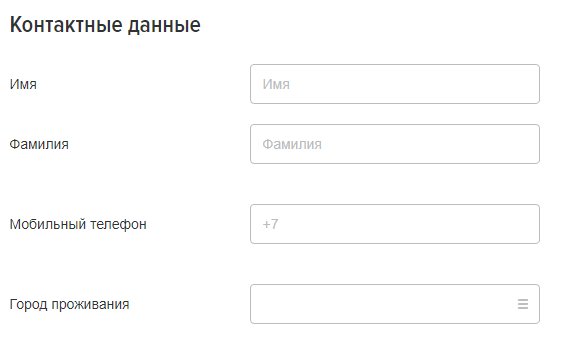
\includegraphics[width=12cm]{images/image14.png}
            \caption{\label{fig:1}%
                Структура пункта контактных данных}
        \end{figure}

    \item Заполнить пункты основной информации. Структура пункта представлена 
    на рисунке~\ref{fig:2}.
        \begin{figure}[!ht]
            \centering
            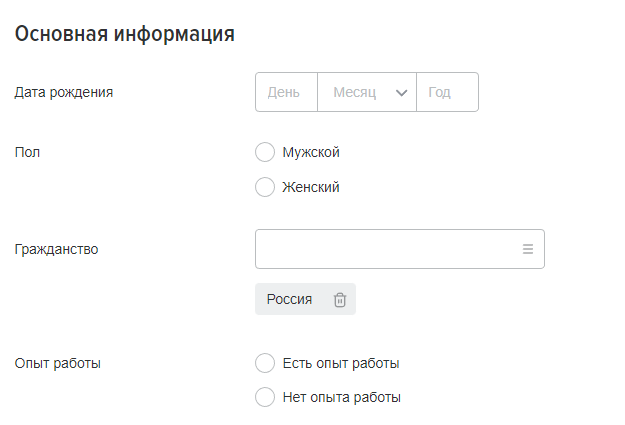
\includegraphics[width=12cm]{images/image12.png}
            \caption{\label{fig:2}%
                Структура пункта основной информации}
        \end{figure}

    \item Указать желаемую специальность и заработную плату. Структура пункта 
    представлена на рисунке~\ref{fig:3}.
        \begin{figure}[!ht]
            \centering
            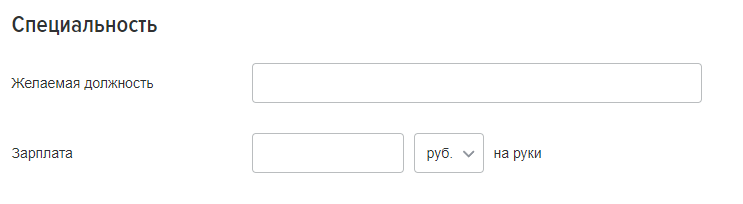
\includegraphics[width=12cm]{images/image3.png}
            \caption{\label{fig:3}%
                Структура пункта специальности}
        \end{figure}

    \item Указать опыт работы (при его наличии), а также навыки, которые 
    предлагаются пользователю в качестве отдельных ключевых слов;
    \item Указать уровень образования, место его получения и года выпуска 
    (либо <<по настоящее время>> для школьников или студентов);
    \item Указать владение языками и его уровень (для иностранных). Структура пункта 
    представлена на рисунке~\ref{fig:4}.
        \begin{figure}[!ht]
            \centering
            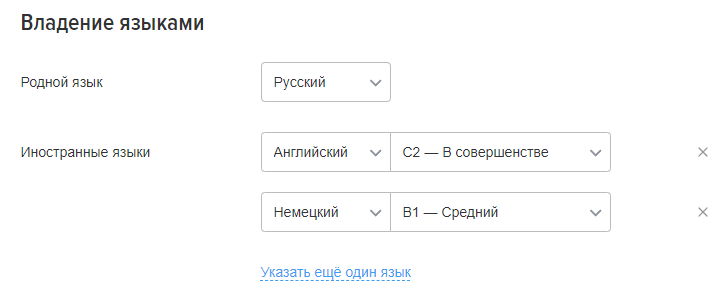
\includegraphics[width=12cm]{images/image1.png}
            \caption{\label{fig:4}%
                Структура пункта владения языками}
        \end{figure}

    \item Пункт <<другой важной информации>> содержит в себе сведения о готовности к переезду, 
    желаемой занятости, графика работы, наличии автомобиля и водительских прав, а также 
    категорий в них. Для иностранных граждан присутствует пункт <<разрешения на работу>>.
\end{enumerate}

После публикации резюме его может быть не видно большинству работодателей, 
если некоторые из пунктов являются незаполненными. Сам алгоритм составления резюме 
не является сложным, а возможность откликнуться на вакансию часто подразумевает 
прикрепление сопроводительного письма помимо самой <<визитки>> соискателя.
Дополнительно сервис hh.ru предлагает услуги экспертов для составления грамотного 
резюме за небольшую плату (от 3 до 8 тысяч рублей в зависимости от разновидности услуги).

\subsection{Сервис для поиска работы в IT-сфере Хабр Карьера}
Являясь одним из популярных в России коллективным IT-блогом, Хабр смог развить не только 
форум для программистов, но и отдельные сервисы, которые связаны с помощью начинающих 
и опытных разработчиков, тестировщиков, дизайнеров и прочих информационных вакансий. 
Одним из подобных сервисов для поддержки начинающих и опытных IT-специалистов является 
Хабр Карьера\cite{Gridneva_2021}.

В отличие от hh.ru, Хабр Карьера публикует вакансии исключительно связанные с IT сферой. 
На сервисе предлагаются вакансии как небольших компаний, так и компаний-гигантов 
(например, Яндекс, Авито, Mail.ru). Для своих коллег и знакомых на Хабр Карьера 
пользователю предоставляется возможность оставить профессиональную рекомендацию.

Составление резюме на сайте начинает свой путь с процесса авторизации на сервисе. 
Это можно сделать как при помощи стандартной регистрации с подтверждением почты, 
так и через сервисы, доступные в России (Вконтакте, Google Account).

Составить своё резюме Хабр Карьера предлагает сразу же после авторизации, 
причём существует возможность импортировать резюме с сервиса hh.ru. Данное окно 
представлено на рисунке~\ref{fig:5}.
\begin{figure}[!ht]
    \centering
    
\includegraphics[width=12cm]{images/image9.png}
    \caption{\label{fig:5}%
        Предложение импорта резюме с hh.ru}
\end{figure}


Для ручного ввода или создания первого резюме пользователю потребуется 3 шага:
\begin{enumerate}
    \item На первом указывается фамилия и имя, пол и дата рождения, а также основная цель 
    регистрации на Хабр Карьера. Структура пункта представлена на рисунке~\ref{fig:6}.
    \begin{figure}[!ht]
        \centering
        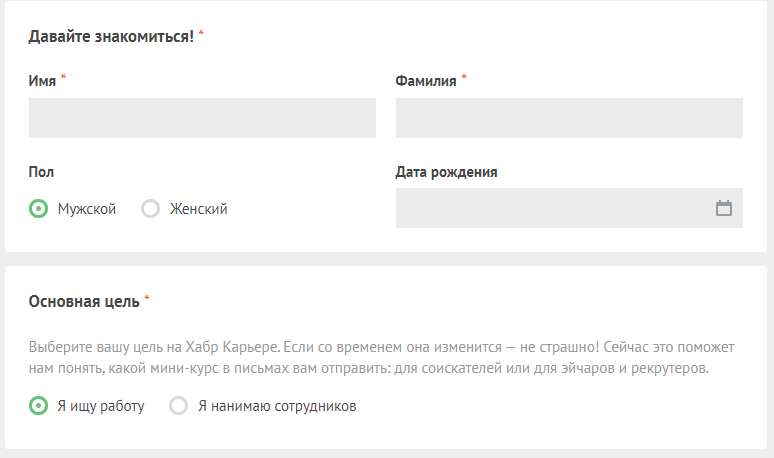
\includegraphics[width=12cm]{images/image15.png}
        \caption{\label{fig:6}%
            Первый шаг регистрации}
    \end{figure}

    В той же вкладке (если выбрана роль соискателя) необходимо выбрать основную 
    специализацию и отдельный профиль, а также квалификация (Intern, Junior, Middle, 
    Senior, Lead). В отличие от hh.ru и в связи с ограниченной сферой деятельности, 
    все специализации представлены наглядно и распределены по категориям для удобства выбора.
    Структура пункта представлена на рисунке~\ref{fig:7}.
    \begin{figure}[!ht]
        \centering
        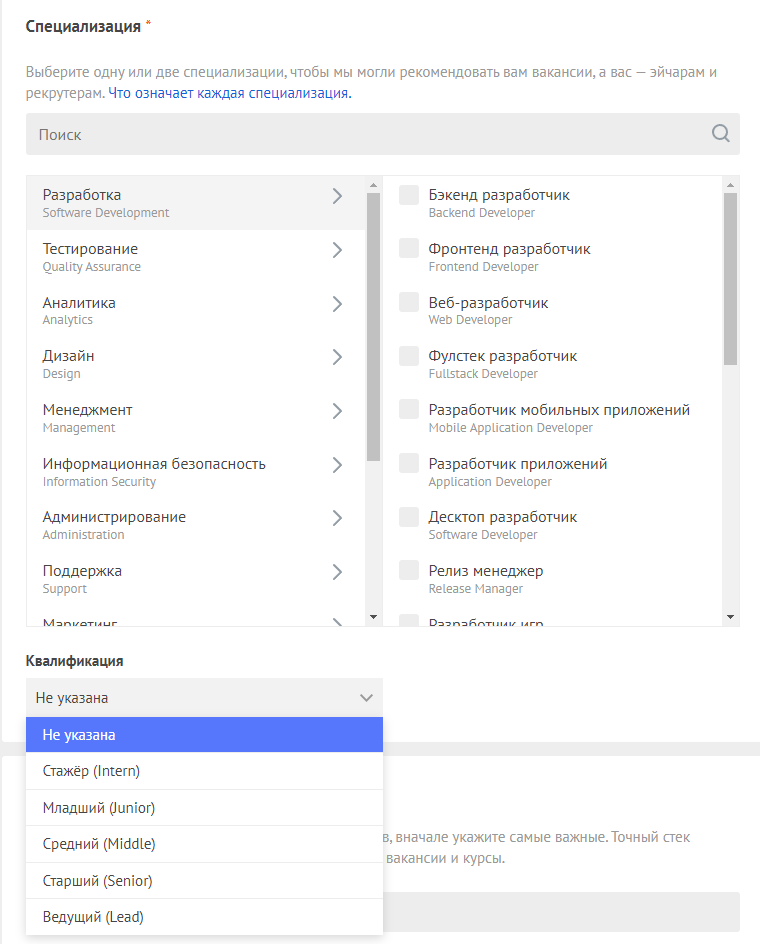
\includegraphics[width=12cm]{images/image6.png}
        \caption{\label{fig:7}%
            Выбор специализации и квалификации}
    \end{figure}

    Дополнительно указываются профессиональные навыки, которым владеет соискатель. 
    Список таких навыков очень обширен и позволяет гибко найти нужные профессиональные 
    <<скиллы>>. Часть из них предлагается уже на старте как <<Самые популярные>>. 
    Структура пункта представлена на рисунке~\ref{fig:8}.
    \begin{figure}[!ht]
        \centering
        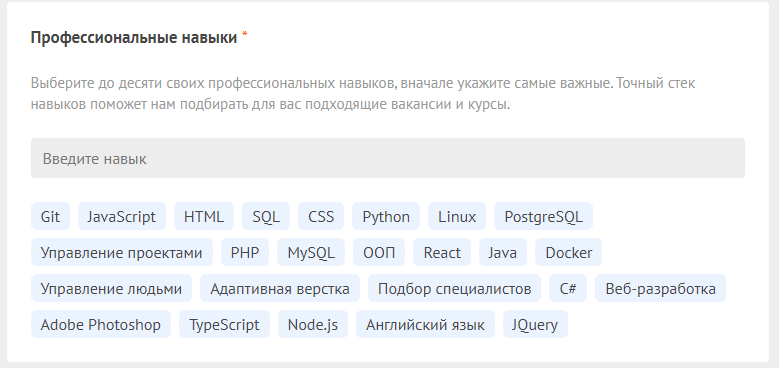
\includegraphics[width=12cm]{images/image19.png}
        \caption{\label{fig:8}%
            Выбор профессиональных навыков}
    \end{figure}

    \item Вторая вкладка будет содержать в себе контактную информацию, что также важно 
    при составлении резюме, ведь одних данных об имени и фамилии будет недостаточно 
    для связи с соискателем. По содержанию оно аналогично сервису hh.ru, например, 
    указать город проживания и пункт о готовности к переезду или удаленной работе. 
    Однако для связи соискатель может оставить не только номер телефона или 
    ссылку-портфолио, но и свой логин в мессенджерах, например, в Telegram.
    Структура пункта представлена на рисунке~\ref{fig:9}.
    \begin{figure}[!ht]
        \centering
        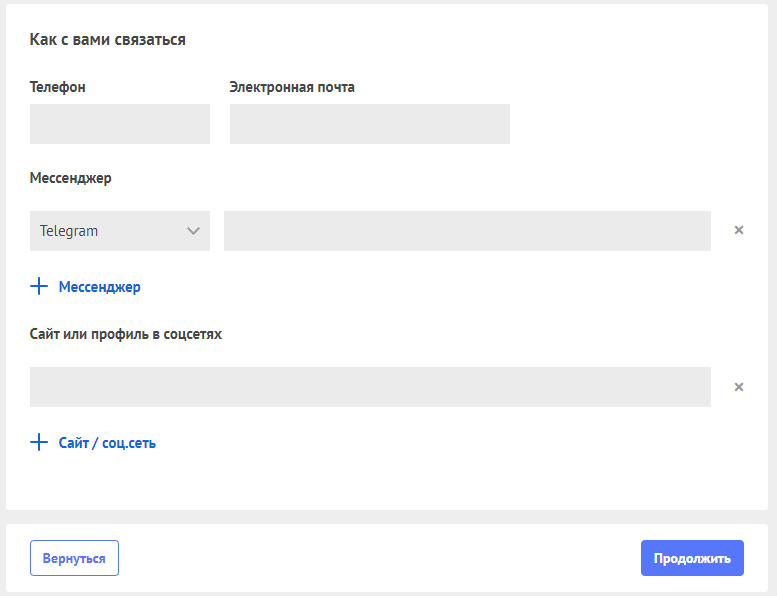
\includegraphics[width=12cm]{images/image2.png}
        \caption{\label{fig:9}%
            Выбор контактных данных}
    \end{figure}

    \item Последняя вкладка содержит в себе пункты, связанные с опытом работы. 
    По статистике, большинство работодателей присматриваются к кандидатам, 
    у которых за спиной есть даже самый незначительный, но указанный в резюме опыт. 
    Однако на Хабр Карьера отсутствует пункт, связанный с <<фрилансом>>, что мешает 
    заполнению опыта работы в данной сфере, но его можно добавить самостоятельно.
\end{enumerate}

\subsection{Международный сервис поиска работы Skipp.dev}
Skipp.dev является международным сервисом как для поиска работы, так и для найма 
работников со стороны работодателей. Различие между предыдущими сервисами отличается 
не только в плане дизайна, но и порядка заполнения пунктов. Для того, чтобы начать 
поиск желаемой вакансии, необходимо также пройти авторизацию, и после этого 
поочередно заполнить пункты специализации и навыков:
\begin{enumerate}
    \item Необходимо верифицироваться по номеру мобильного телефона. 
    Этот пункт необходим для того, чтобы проверить подлинность аккаунта, 
    а также для дальнейшей авторизации на сервисе при помощи смс-кода.
    \item На первом шаге соискателю предлагается выбрать свои навыки. Структура 
    пункта представлена на рисунке~\ref{fig:10}.
        \begin{figure}[!ht]
            \centering
            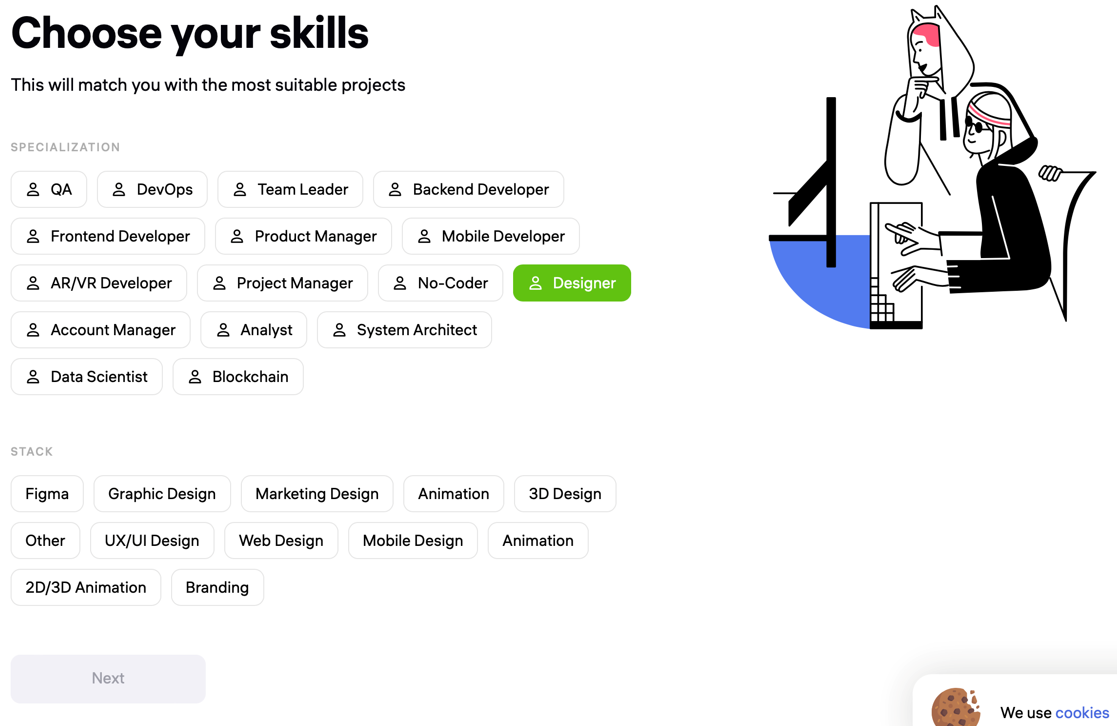
\includegraphics[width=12cm]{images/image10.png}
            \caption{\label{fig:10}%
                Выбор навыков}
        \end{figure}

    \item После выбора навыков необходимо указать уровень навыков, 
    которые были выбраны на предыдущей странице, что является нестандартным 
    для отечественных сервисов. Структура пункта представлена на рисунке~\ref{fig:11}.
    \begin{figure}[!ht]
        \centering
        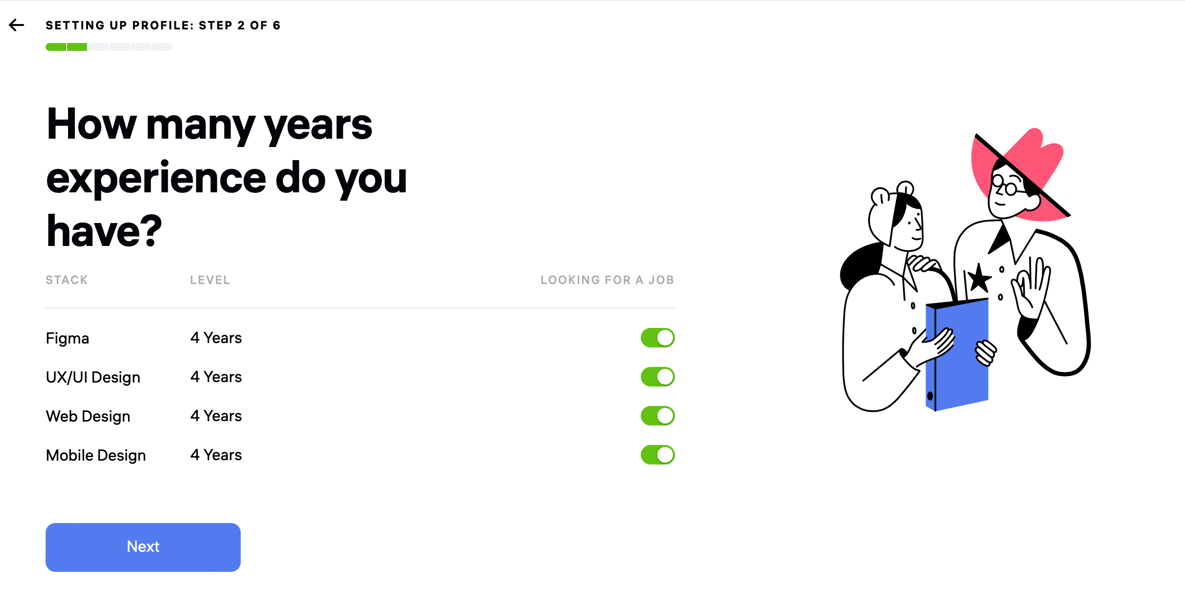
\includegraphics[width=12cm]{images/image11.png}
        \caption{\label{fig:11}%
            Выбор уровня навыков}
    \end{figure}

    \item Заполнение опыта работы не сильно отличается от рассмотренных 
    нами предыдущих платформ, но имеет свои преимущества. Например, 
    для более подробного описания должностных обязанностей на предыдущих 
    местах работы пользователю предлагаются различные виды деятельности, 
    также начиная с самых популярных на сайте. Также к опыту работы есть возможность 
    приложить изображения в качестве портфолио. Структура пункта представлена 
    на рисунке~\ref{fig:12}.
    \begin{figure}[!ht]
        \centering
        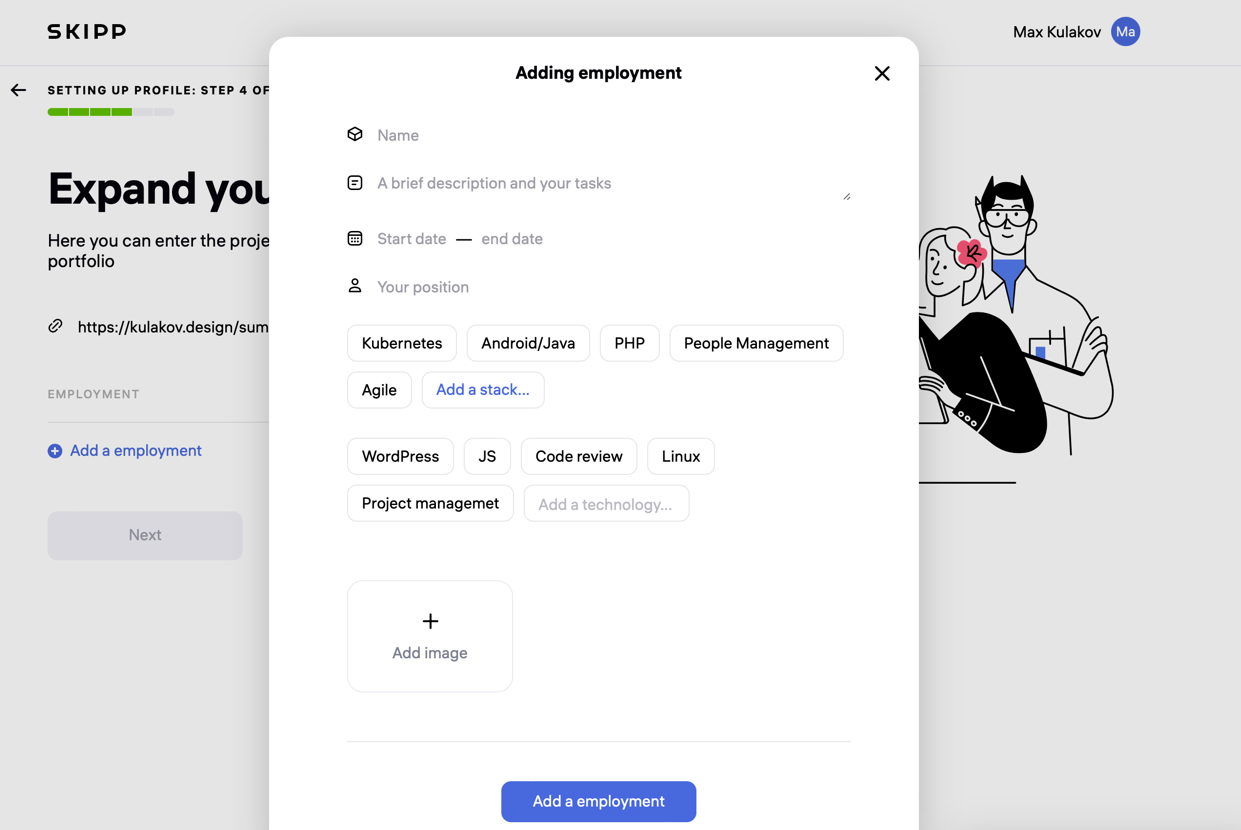
\includegraphics[width=12cm]{images/image17.png}
        \caption{\label{fig:12}%
            Выбор опыта работы}
    \end{figure}

    \item Последний пункт содержит в себе форму заполнения контактной информации, 
    начиная от ФИО до номера телефона и e-mail. 
\end{enumerate}

Из положительных сторон данного сервиса можно выделить приятный внешний вид 
и неторопливое пошаговое заполнение всех пунктов. Акцент делается на опыте работы, 
чтобы сконцентрировать внимание пользователя на том, как будет лучше преподнести 
себя будущим работодателям. Однако сервис не захватывает резюме с других платформ, 
что делает эту платформу абстрагированной от других себе подобных.

\subsection{Карьерный ресурс Icanchoose}
ICanChoose рекомендует себя в качестве карьерного ресурса нового формата. Из новизны, 
предполагаемо, сервис предлагает помощь в поиске работы, а также предлагает карьерные советы.

Авторизация на сервисе доступна при помощи ВКонтакте, а так же с email.
При создании резюме сразу предлагается импорт из сервиса hh.ru, представленный 
на рисунке~\ref{fig:13}.
\begin{figure}[!ht]
    \centering
    
\includegraphics[width=12cm]{images/image13.png}
    \caption{\label{fig:13}%
        Возможность импорта резюме}
\end{figure}

Процесс составления резюме происходит так же, как на вышерассмотренных сервисах, 
но с добавлением пунктов о хобби, достижениях и сопроводительное письмо. 
Также на сервисе существует возможность предварительного просмотра готового резюме, 
которое работает только при полном заполнении основной информации.

\subsection{Веб-сервис для хостинга ГитХаб}
ГитХаб зарекомедовал себя крупнейшим сервисом для хостинга с возможностью их совместной 
разработки, но, благодаря своим инструментам, на платформе возможно создание резюме. 
На аккаунте начинающего разработчика такое решение будет являться хорошим продолжением 
стратегии его развития, так как при рассмотрении профиля в качестве портфолио работодателю 
будут видны все разработанные проекты, на основе чего высока вероятность получить 
приглашение самому разработчику.

Для начала работы с составлением резюме пользователю необходимо создать новый репозиторий 
с названием, которое будет повторять <<юзернейм>> на GitHub. Сервис подчеркнёт его в качестве 
уникального и захватит его нужным образом.

Вся информация по резюме будет находиться в файле README.md. Другими словами, 
всё написанное и отформатированное будет видно на странице в GitHub и будет служить 
в дальнейшем красочной визиткой для тех, кто будет просматривать профиль 
разработчика\cite{gh_cv}.

Удобство написания резюме в GitHub подкрепляется отсутствием шаблона и полной свободой мысли, 
однако из-за отсутствия точных критериев содержания информации необходимо для себя составлять 
структуру будущей визитки, чтобы она выглядело не только гармонично, 
но и понятно.

\subsection{Блочный конструктор веб-сайтов Tilda}
Tilda изначально является конструктором, позволяющиим на внутренних шаблонах создать 
любой сайт, который удовлетворяет задаче, в том числе резюме. Для последнего на сайте 
есть готовые шаблоны, которые упрощают работу с сервисом, 
в частности для начинающих пользователей\cite{tilda_template}. 
Визуально это представлено на рисунке~\ref{fig:14}.
\begin{figure}[!ht]
    \centering
    
\includegraphics[width=12cm]{images/image7.png}
    \caption{\label{fig:14}%
        Предложение использования шаблона}
\end{figure}

Составленный из блоков шаблон также можно будет использовать в качестве собственного лендинга.

Профиль на Тильде также является портфолио, что позволяет работодателю, желающему создать 
сайт на данном сервисе, найти необходимого ему разработчика при помощи системы 
заказов на Tilda Express.

Резюме на Tilda Express представляет из себя небольшую страницу с размещенными на 
них проектами, разработанными на Tilda, а также окошком с заполнением заявки на обратную 
связь при наличии желания заказать у данного разработчика собственный сайт. Пример резюме 
представлен на рисунке~\ref{fig:15}.
\begin{figure}[!ht]
    \centering
    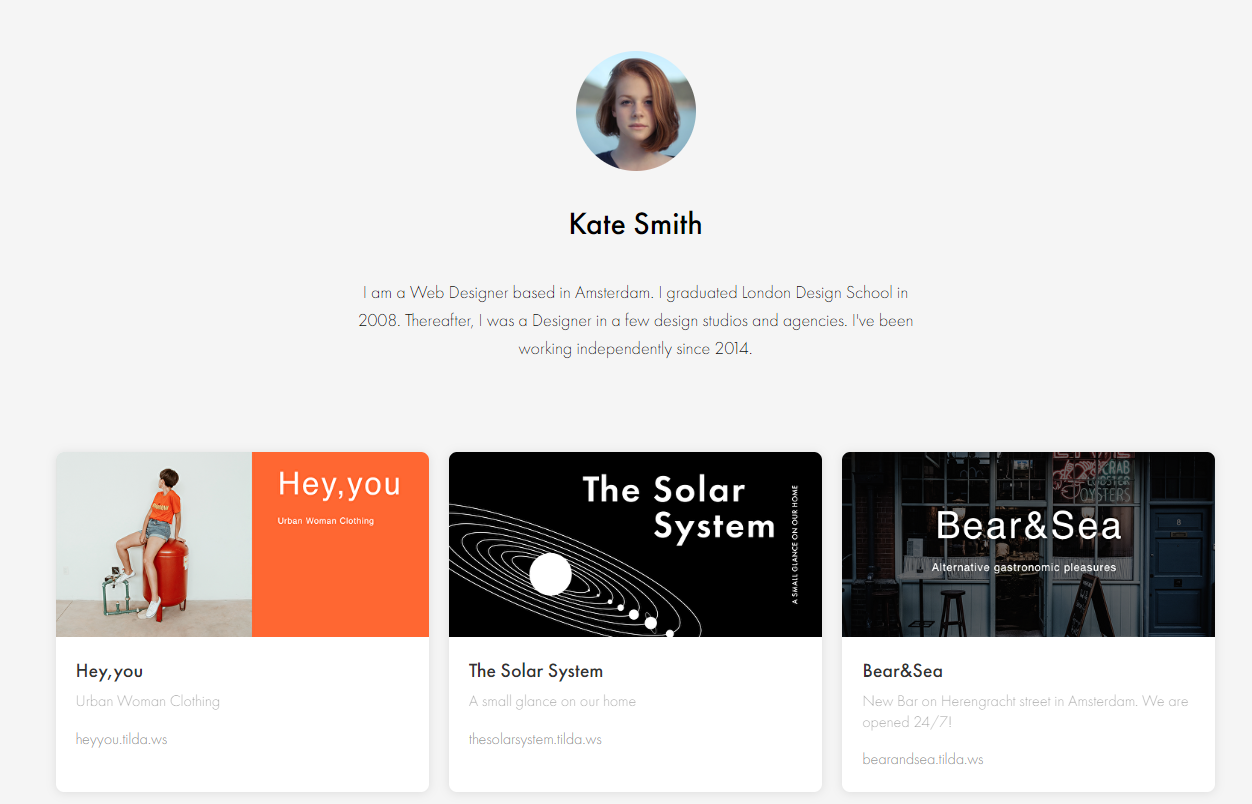
\includegraphics[width=12cm]{images/image8.png}
    \caption{\label{fig:15}%
        Пример резюме на платформе Tilda}
\end{figure}

\subsection{Онлайн-конструктор резюме Simpledoc}
SimpleDoc является сервисом исключительно по составлению резюме. На сайте предлагается 
составление резюме в трёх основных этапах: заполнение формы, выбор дизайна для резюме 
и его скачивание или отправка по e-mail, представленных на рисунке~\ref{fig:16}.
\begin{figure}[!ht]
    \centering
    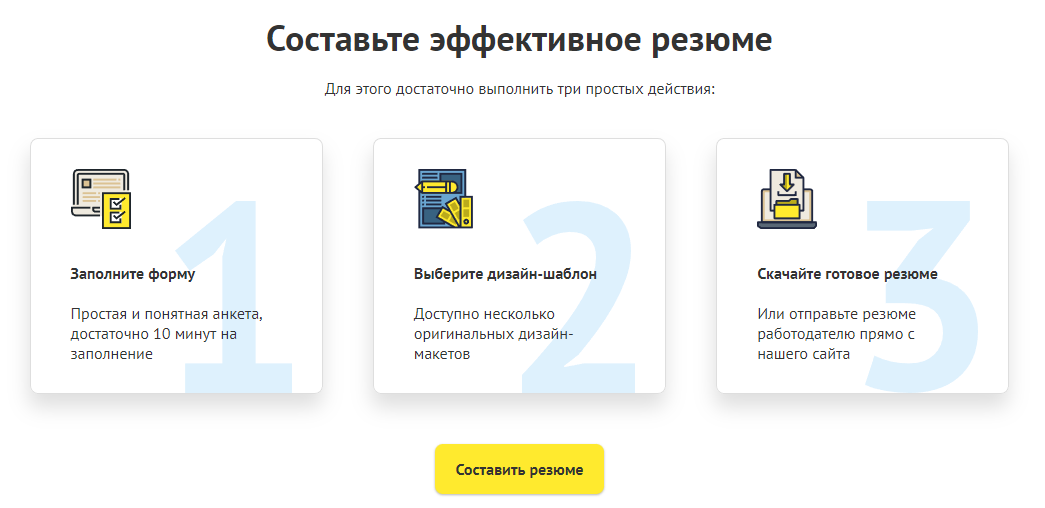
\includegraphics[width=12cm]{images/image5.png}
    \caption{\label{fig:16}%
        Этапы создания резюме}
\end{figure}

Сам процесс заполнения формы занимает около 10ти минут и содержит в себе стандартные 
для резюме пункты:
\begin{enumerate}
    \item Основная информация;
    \item Личная информация;
    \item Опыт работы;
    \item Образование;
    \item Курсы и тренинги;
    \item Иностранные языки и компьютерные навыки;
    \item Дополнительная информация.
\end{enumerate}

После заполнения пунктов сервис предлагает выбрать один из четырёх шаблонов 
для дальнейшего скачивания, представленных на рисунке~\ref{fig:17}.
\begin{figure}[!ht]
    \centering
    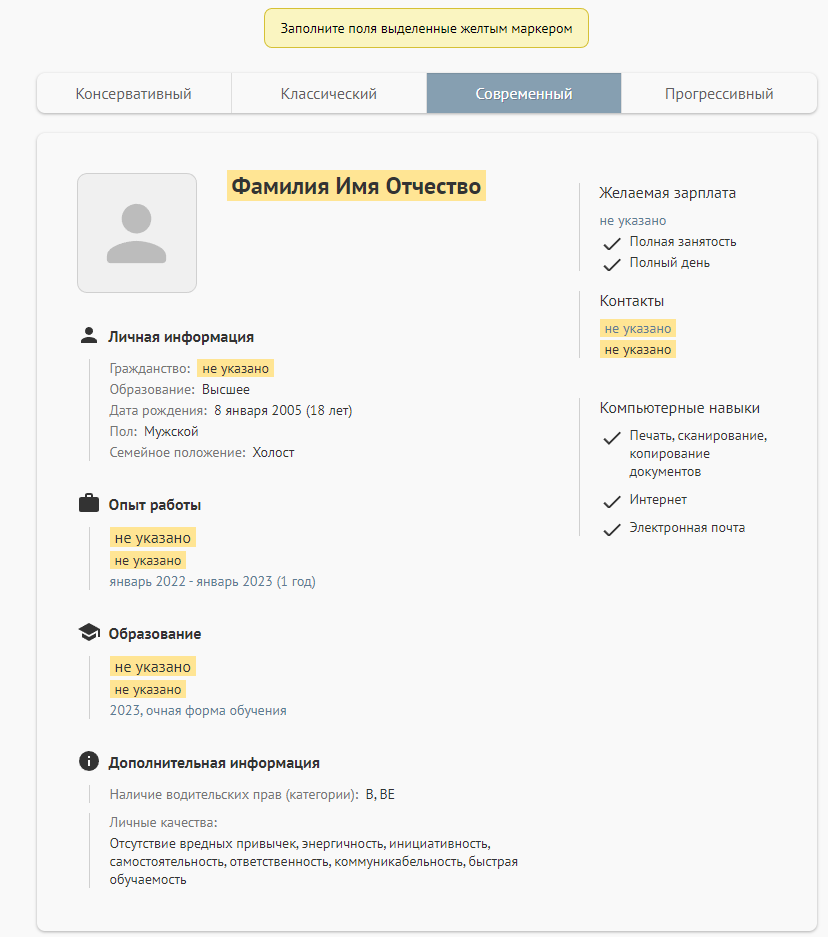
\includegraphics[width=12cm]{images/image4.png}
    \caption{\label{fig:17}%
        Вариант шаблона резюме}
\end{figure}

После составления резюме по шаблону пользователь сможет скачать его и редактировать 
в течение месяца после разовой оплаты на самом сервисе.
Сервис также не позволяет импортировать резюме с других сервисов.

\subsection{Онлайн-конструктор Enhancv}
Enhancv также является сервисов для составления резюме, но в отличие от SimpleDoc 
имеет приятный дизайн, представленный на рисунке~\ref{fig:18} уже со стартовой страницы:
\begin{figure}[!ht]
    \centering
    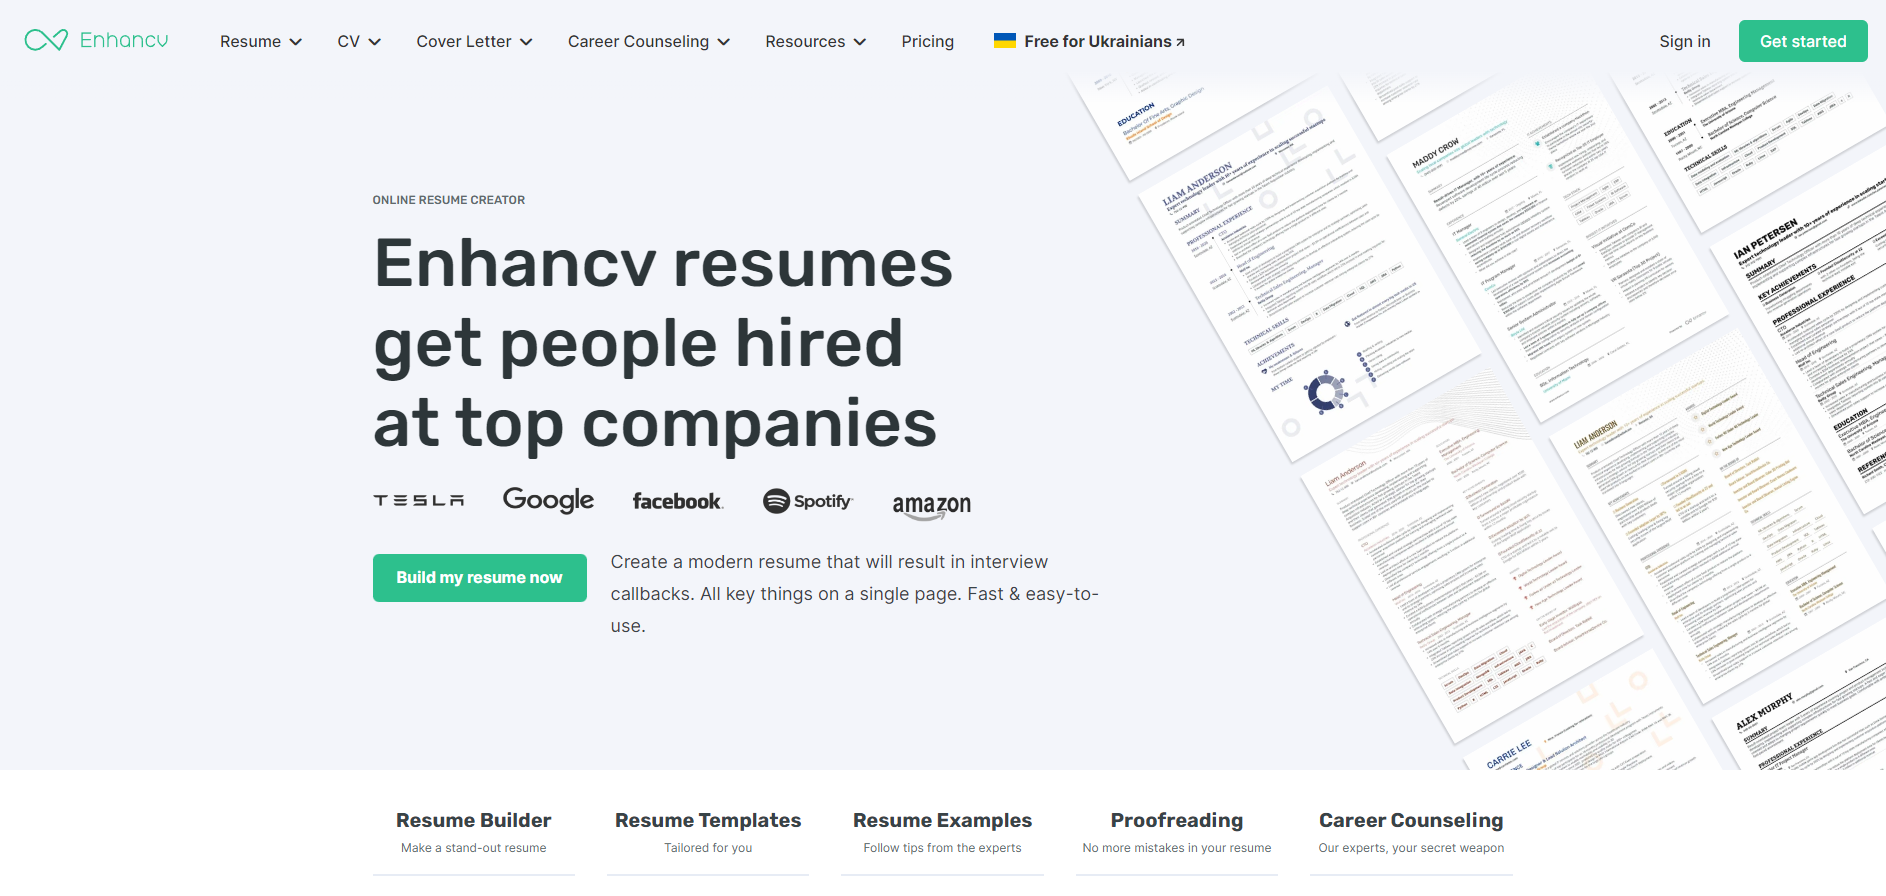
\includegraphics[width=12cm]{images/image18.png}
    \caption{\label{fig:18}%
        Внешний вид сервиса Enhancv}
\end{figure}

При начале работы нам помогает <<виртуальный>> помощник, показанный на рисунке~\ref{fig:19}, 
с которым мы заполняем пункты по очереди:
\begin{enumerate}
    \item Имя Фамилия
    \item Наличие опыта в создании резюме (для возможности его импортировать)
    \item Готовые шаблоны для будущего резюме.
\end{enumerate}

\begin{figure}[!ht]
    \centering
    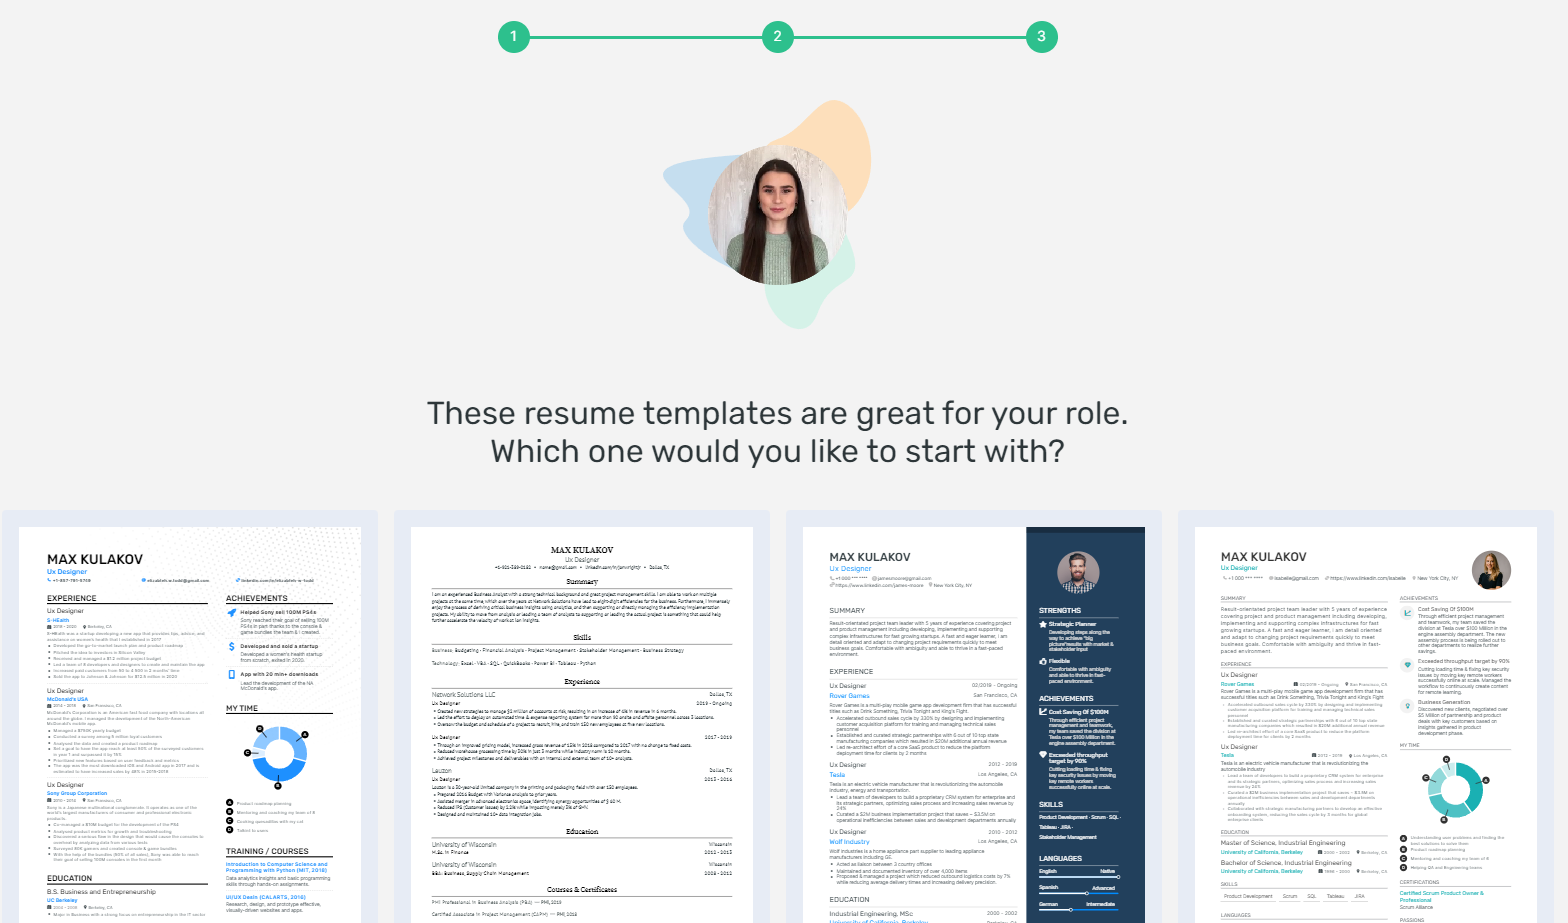
\includegraphics[width=12cm]{images/image16.png}
    \caption{\label{fig:19}%
        Помощник в составлении резюме}
\end{figure}

После чего предлагается отредактировать информацию в резюме напрямую в одном из шаблонов, 
показанном на рисунке~\ref{fig:20}:
\begin{figure}[!ht]
    \centering
    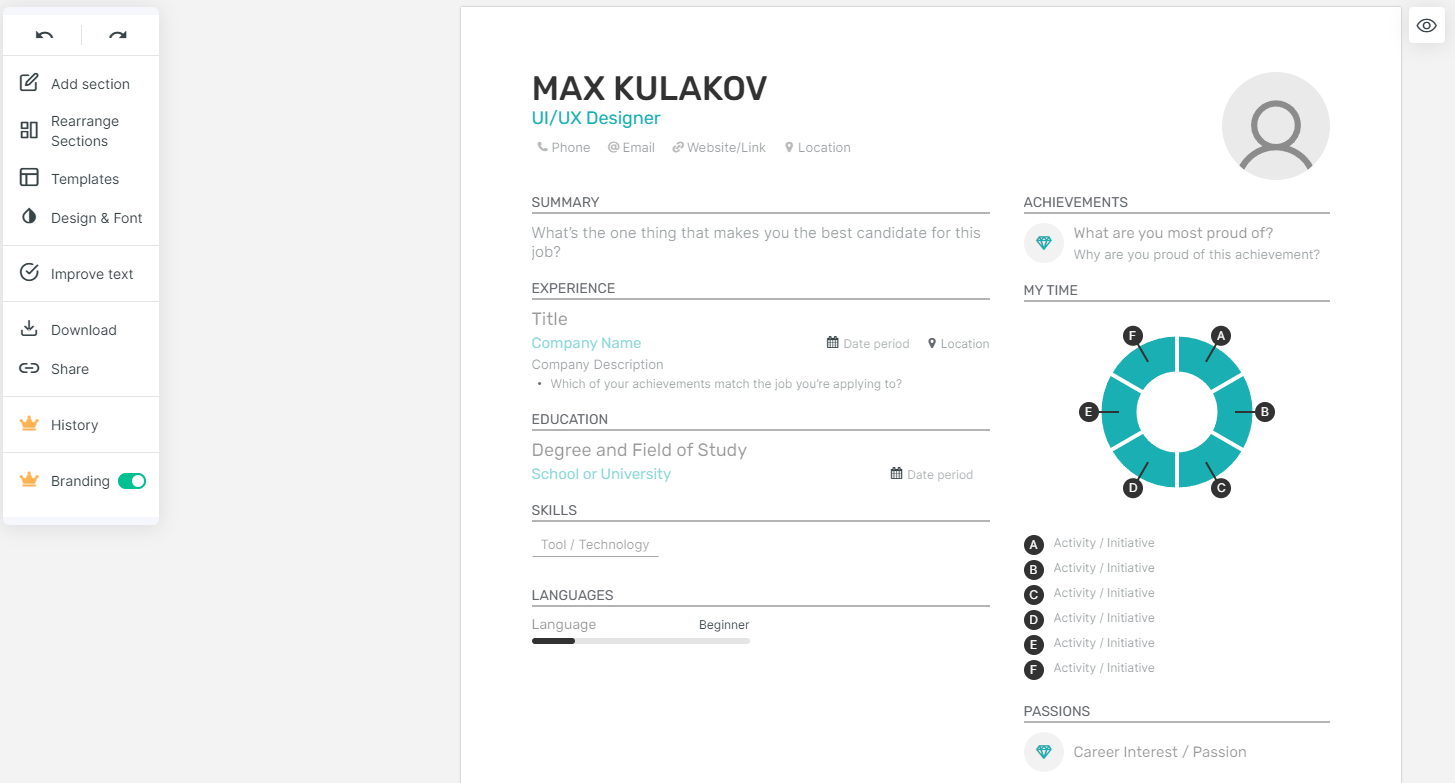
\includegraphics[width=12cm]{images/image20.png}
    \caption{\label{fig:20}%
        Внешний вид шаблона резюме}
\end{figure}

На выбор предлагается множество инструментов для комфортной работы с шаблоном: 
от возможности редактирования шрифта до редактируемой инфографики. 
Также является платным сервисом.

На основе просмотренных конкурентных платформ можно вынести их основные недостатки:
\begin{enumerate}
    \item Не все сервисы предлагают импорт резюме из других платформ;
    \item Сервисы, работающие исключительно на составление резюме, берут деньги за свои услуги;
    \item Некоторые сервисы при указании опыта работы требуют официальное название 
    компании или должности, даже если они не зарегистрированы, 
    и не всегда удается указать нужное название;
    \item В дополнение к пункту 3, не везде возможно указание опыта <<свободных заказов>> 
    вне сервисов по типу <<Фриланс.ру>>
    \item Для русскоязычного сегмента сервисов поиска работы основным является именно 
    HeadHunter, импорт резюме с которого предлагается лишь в части платформ.
\end{enumerate}



% Практическая часть


\section{Основные аспекты разработки платформы единого резюме}
С учётом собранных данных при анализе научной литературы и конкурентных сервисов 
для разработки собственной платформы единого резюме необходимо придерживаться следующим пунктам:
\begin{enumerate}
    \item Реализовать сбор информации о текущих резюме с уже существующих сервисов;
    \item Предоставить возможность объединения, замены, дополнения или удаления 
    смежных или отсутствующих пунктов данных;
    \item Создание единого бланка с отредактированными или созданными полями, 
    с возможностью хранения их на личном пространстве;
\end{enumerate}

Для составления базового и необходимого на начальное время функционала, в качестве развития 
платформы единого резюме, следует реализовать следующее:
\begin{enumerate}
    \item Удобный пользовательский интерфейс, соответствующий современным web-стандартам 
    и позволяющий пользоваться функционалом сервиса на любом устройстве, поддерживающим 
    работу с браузерами;
    \item Возможность создания пользователем персональной страницы на основе шаблонов, 
    для возможности доступа к актуальному резюме при переходе по ссылке сервиса;
    \item Возможность переноса резюме из стороннего ресурса в шаблон платформы;
    \item Публикацию серверного проекта на хостинг, поддерживающий динамическое 
    создание и обновление страниц согласно подготовленным данным.

\end{enumerate}


\subsection{Создание прототипа платформы резюме}
Прототипирование – разработка интерактивной модели приложения, симулирующее коммуникацию 
пользователя с интерфейсом и созданное для тестирования базового функционала. 
Данный этап необходим чтобы удобно и корректно выстроить логику взаимодействия с продуктом 
и достижения поставленной задачи.

Для создания прототипа использовано приложение Figma, так как оно является бесплатным 
(платная версия отличается от бесплатной количеством единовременных редакторов проекта 
и невозможностью организовать команду) и полностью подходит для реализации данного 
этапа разработки. Были изображены экраны бланка, страницы ввода и свободного
редактора контента, показанные на рисунке~\ref{fig:21}.

\begin{figure}[!ht]
    \centering
    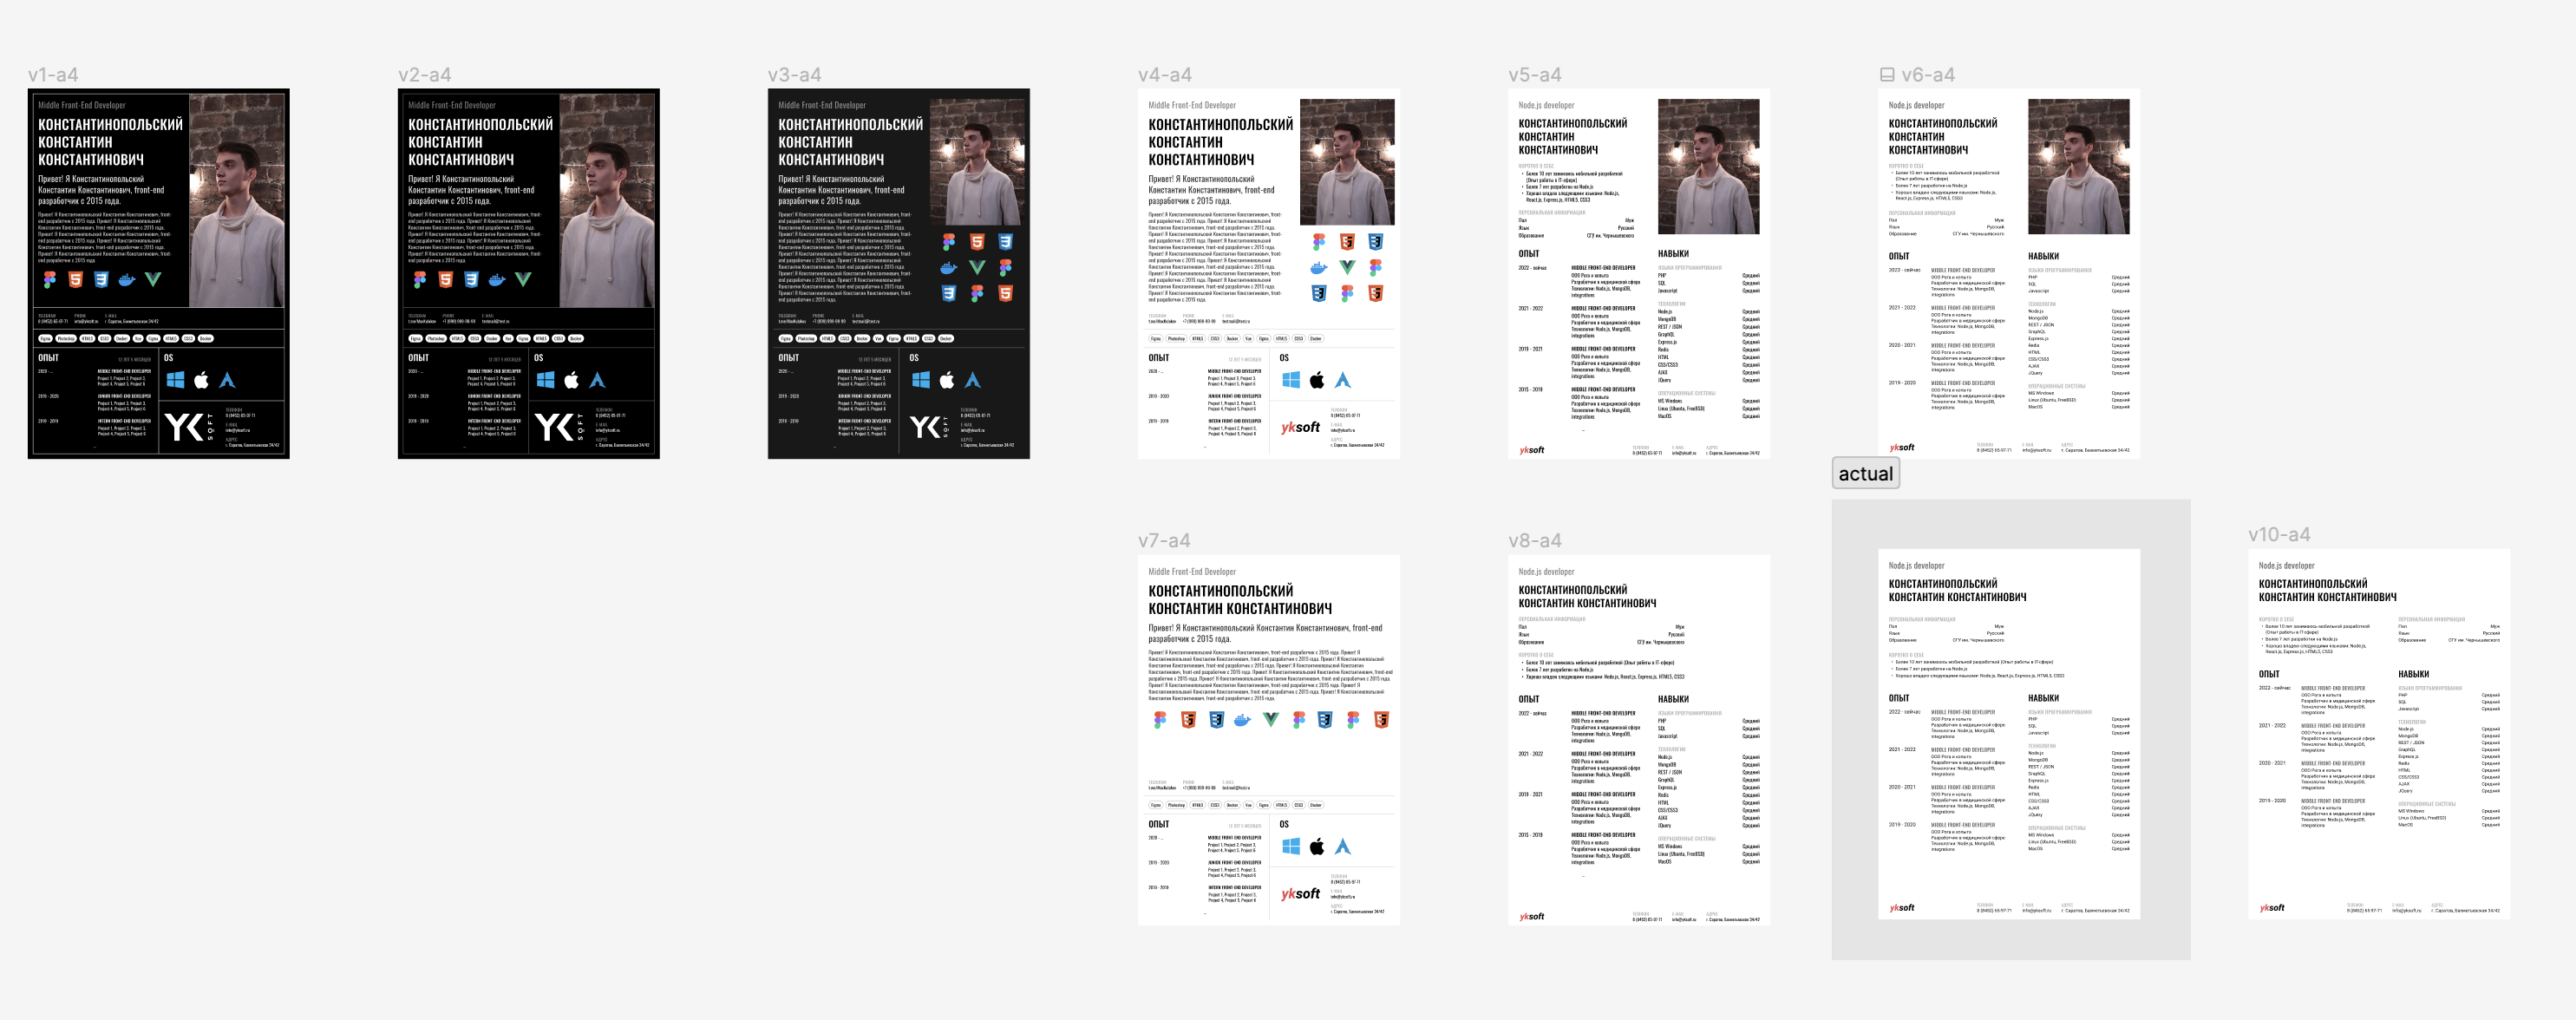
\includegraphics[width=12cm]{images/image21.png}
    \caption{\label{fig:21}%
        Внешний вид прототипов платформы}
\end{figure}

Далее идёт проверка прототипа на реальных людях, проведённая коридорным 
тестированием – перед случайными людьми ставится задача взаимодействовать 
с интерфейсом приложения, тогда как разработчик убеждается 
в корректности задуманного поведения и находит ошибки. 
Такие тесты помогают максимально быстро получить обратную связь, потратив
минимальное количество времени на поиск респондентов.
Результатом тестирования стало подтверждение правильности
разработанного прототипа, поэтому можно перейти к увеличению 
детализации экранов и написанию кода. Важным аспектом при разработке прототипа
было сохранение адаптивности страницы, чтобы контент вписывался в различные разрешения
экрана и кроме того мог быть адаптирован под печатную версию в формате А4.


\subsection{Настройка рабочей среды}
Создание приложения происходило на компьютере под управлением Mac OS, 
что позволяет использовать Terminal – средство взаимодействия с системой 
посредством командной строки при помощи bash-команд. В качестве среды 
разработки был выбран Visual Studio Code – легковесный текстовый редактор
для кроссплатформенной разработки.

С помощью терминала установим пакетный менеджер Homebrew, который необходим 
для загрузки и запуска компонентов системы. Сделать это можно с помощью команды:

\begin{minted}[fontsize=\small, breaklines=true, style=bw, linenos]{bash}
/bin/bash -c "$(curl -fsSL https://raw.githubusercontent.com/Homebrew/install/ HEAD/install.sh)"
\end{minted}

Для работы с библиотеками разрабатываемой платфрмы необходимо выполнить установку Node.js – 
среды запуска Java Script приложений и Watchman – утилиты для контроля изменений файлов:

\begin{minted}[fontsize=\small, breaklines=true, style=bw, linenos]{bash}
brew install node
brew install watchman
\end{minted}


Инициализируем проект, создав стартовое рабочее приложение:

\begin{minted}[fontsize=\small, breaklines=true, style=bw, linenos]{bash}
mkdir cv-editor
cd cv-editor
npm init
\end{minted}


После перехода в папку проекта и инициации проекта необходимо добавить
требуемые зависимости, такие как parcel, необходимый для итоговой сборки и 
работы в режиме сервера и editor.js, необходимый для использования 
возможностей динамического ввода и сохранения инфомрации пользователя:
\begin{minted}[fontsize=\small, breaklines=true, style=bw, linenos]{bash}
yarn add --dev parcel
yarn add @editorjs/editorjs
\end{minted}


\subsection{Реализация клиентской части платформы}
Входным файлом проекта назначим index.html. Опишем его стандартную структуру и 
внутрь тега head добавим ссылки на файл стилей main.css и файл шрифта Mona-Sans.woff2 и
стили библиотеки Bootstrap:
\begin{minted}[fontsize=\small, breaklines=true, style=bw, linenos]{html}
<title>CV Editor</title>
<link rel="stylesheet" href="css/main.css">
<link rel="preload" href="./src/font/Mona-Sans.woff2" as="font" type="font/woff2">
<link href="bootstrap.min.css" rel="stylesheet">
\end{minted}


В том же файле добавим блок вызова редактора, кнопку сохранения введённых данных 
и после в конец файла перед закрытием тега body подключим файл скриптов 
проекта index.js и ссылку на файл скриптов библиотеки стилей:
\begin{minted}[fontsize=\small, breaklines=true, style=bw, linenos]{html}
<div id="editorjs"></div>
<button type="button" id="saveButton">Save</button>
<script src="./index.js" type="module"></script>
<script src="bootstrap.bundle.min.js"></script>
\end{minted}


После краткого описания языка разметки нам необходимо реализовать функционал редактора.
Для этого в файле index.js импортируем саму библиотеку и вспомогательные модули для 
отображения и работы с заголовками и стилями. Для описания самого редактора создадим
новый объект редактора, включяющий в себя вышеописанные библиотеки:
\begin{minted}[fontsize=\small, breaklines=true, style=bw, linenos]{js}
import EditorJS from '@editorjs/editorjs'; 
import Header from '@editorjs/header'; 
import List from '@editorjs/list'; 

const editor = new EditorJS({ 
  holder: 'editorjs', 
  tools: { 
    header: {class: Header, inlineToolbar: ['link']}, 
    list: {class: List, inlineToolbar: true},
  }, 
});
\end{minted}


Для использования введённой пользователем информации из блока редактора реализуем функцию
получения данных по нажатию кнопки сохранения. Для этого создадим обработчик события,
находящего элемент на странице по идентификационному значению и через него вызовем 
метод сохранения. Чтобы избежать падения сервера опишем обработчик исключений, возвращающий
данные в случае успешного выполнения и выводящий ошибку в случае воможного возникновения
проблем:
\begin{minted}[fontsize=\small, breaklines=true, style=bw, linenos]{js}
document.getElementById("saveButton").onclick = function() {
  editor.save().then((outputData) => {
    console.log('Article data: ', outputData)
  }).catch((error) => {
    console.log('Saving failed: ', error)
  });
};   
\end{minted}

Создадим заголовок страницы, добавим классы для корректного позиционирования 
кнопок на странице с помощью библиотеки Bootstrap. Для этого создадим тег с классом
контенйера и внутренними отступами с помощью классов container и p-4. Добавим краткую
подсказку для запуска проекта на время разработки и стилизуем кнопку: btn 
btn-outline-primary. Итоговый вид и функционал редактора показан на рисунке~\ref{fig:22}.
\begin{figure}[!ht]
    \centering
    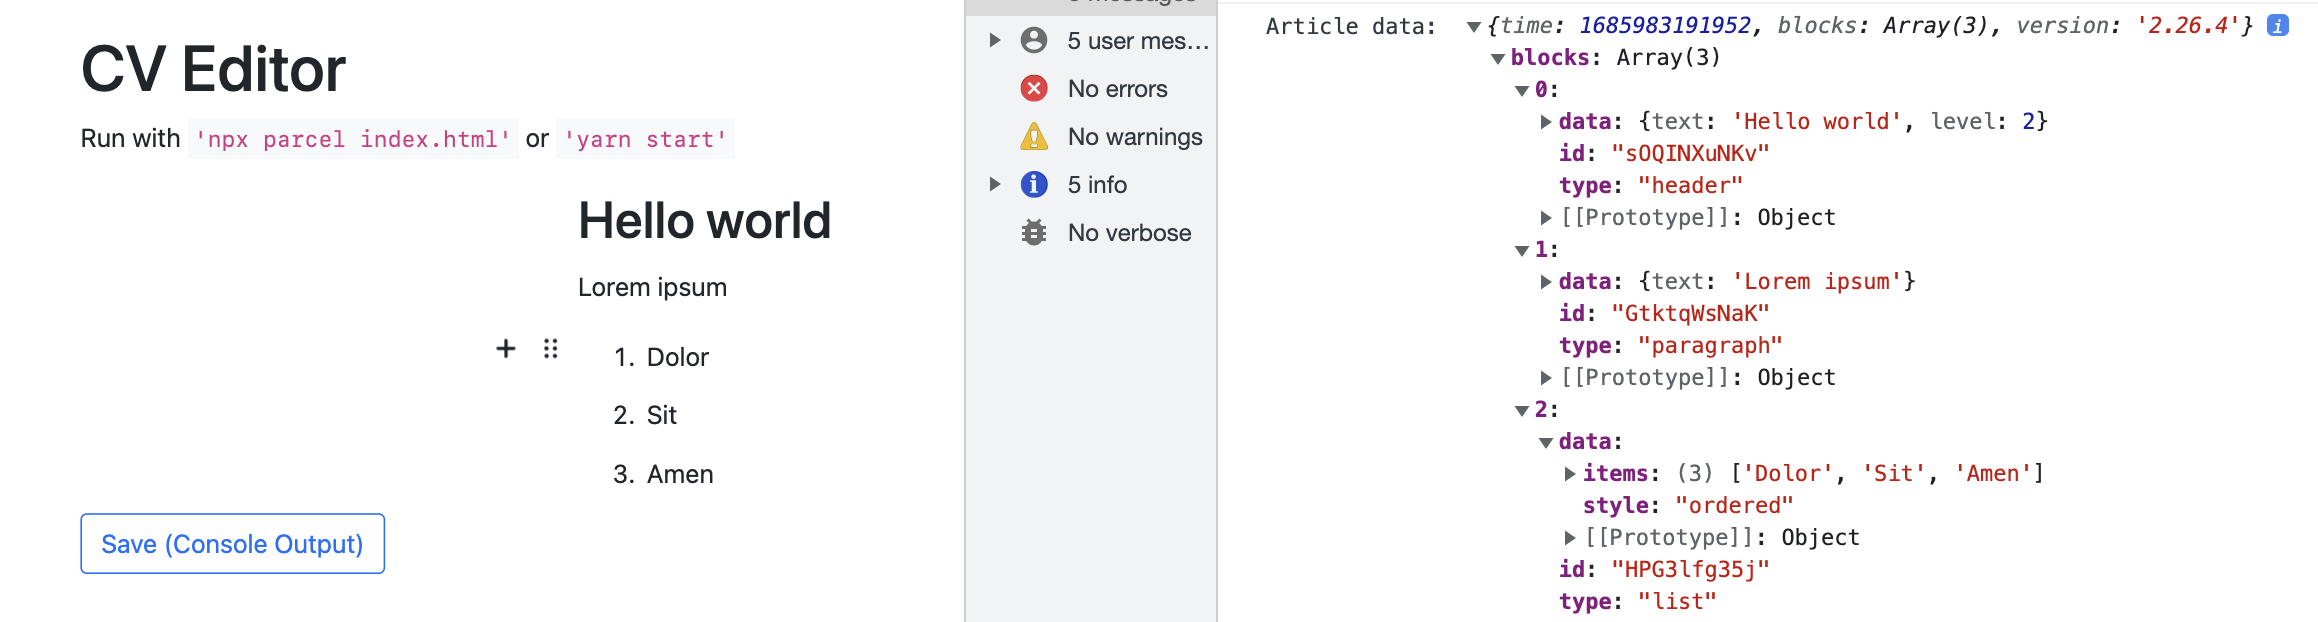
\includegraphics[width=12cm]{images/image22.png}
    \caption{\label{fig:22}%
        Внешний вид свободного редактора данных}
\end{figure}


Реализуем вкладки для шаблона с двумя экранами: заполненным резюме и полями ввода. Для
этого внутрь контейнера добавим список из двух значений, добавим им атрибуты вкладок и 
обозначим первый таб за активный, чтобы при заходе на страницу платформы бланк
загружался сразу.
\begin{minted}[fontsize=\small, breaklines=true, style=bw, linenos]{html}
<div class="container p-4">
    <ul class="nav nav-tabs" id="myTab" role="tablist">
        <li class="nav-item" role="presentation">
        <button class="nav-link active" id="home-tab" data-bs-toggle="tab" data-bs-target="#home" type="button" role="tab" aria-controls="home" aria-selected="true">CV Template</button>
\end{minted}

Согласно дизайну сверстаем шаблон и предусмотрим адаптивное отображение страницы, 
чтобы сайт корректно показывался как на смартфонах, так и на планшетах и компьюетрах.
Для этого необходимо правильно описать стили в классах тегов – от наименьшего или
стандартного разрешения к самому большому. 
\begin{minted}[fontsize=\small, breaklines=true, style=bw, linenos]{html}
<h5 class="h5 text-uppercase text-secondary mt-5">
<strong>Персональная информация</strong></h5>
<div class="row">
    <div class="col-6 col-lg-3">
        Пол
    </div>
    <div class="col-6 col-lg-3 text-end">
        Муж
    </div>
</div>
<div class="row">
    <div class="col-6 col-lg-3">
        Язык
    </div>
    <div class="col-6 col-lg-3 text-end">
        Русский
    </div>
</div>
\end{minted}

Дополнительно для удобства вёрстки
воспользуемся сеткой, представляющей из себя вертикальные направляющие, делящие 
html-страницу на равные части относительно центра страницы с равными отступами от краёв
экрана и равным отступом между колонками. Так на компьютерах с разрешением 1920 пикселей
боковой отступ будет составлять 365 пикселей, размер рабочего контейнера – 1190 пикселей,
всего будет 12 колонок с расстонием между ними в 30 пикселей. Помимо этого внутренние 
контейнеры также адаптивно делятся в своих пропорциях, образуя сетку в сетке.
Итоговый вид шаблона и первой вкладки показан на рисунке~\ref{fig:23}.
\begin{figure}[!ht]
    \centering
    
\includegraphics[width=12cm]{images/image23.png}
    \caption{\label{fig:23}%
        Отображение вкладки переключения и шаблона}
\end{figure}


После вёрстки бланка резюме необходимо реализовать ручные поля ввода, из которых будет
приходить информация для страницы. Разобьём их по категориям и представим
пользователю в доступном виде, необходимом для последовательного заполнения. Для
этого воспользуемся оформлением стилей из библиотеки Bootstrap и реализуем однострочные, 
многострочные поля ввода и селекторы, в которых изначально предложены варианты
выбора данных и стандартное значение.
\begin{minted}[fontsize=\small, breaklines=true, style=bw, linenos]{html}
<h3 class="h3 pb-2">Personal information</h3>
    <div class="row g-4 pb-4">
        <div class="col-md">
            <div class="form-floating">
                <select class="form-select" id="floatingSelectGrid">
                    <option selected>Select</option>
                    <option value="1">Male</option>
                    <option value="2">Female</option>
                </select>
                <label for="floatingSelectGrid">Gender</label>
            </div>
        </div>
\end{minted}

Результатом написания данного блока является вкладка с множеством полей ввода, 
показанных на рисунке~\ref{fig:24}.
\begin{figure}[!ht]
    \centering
    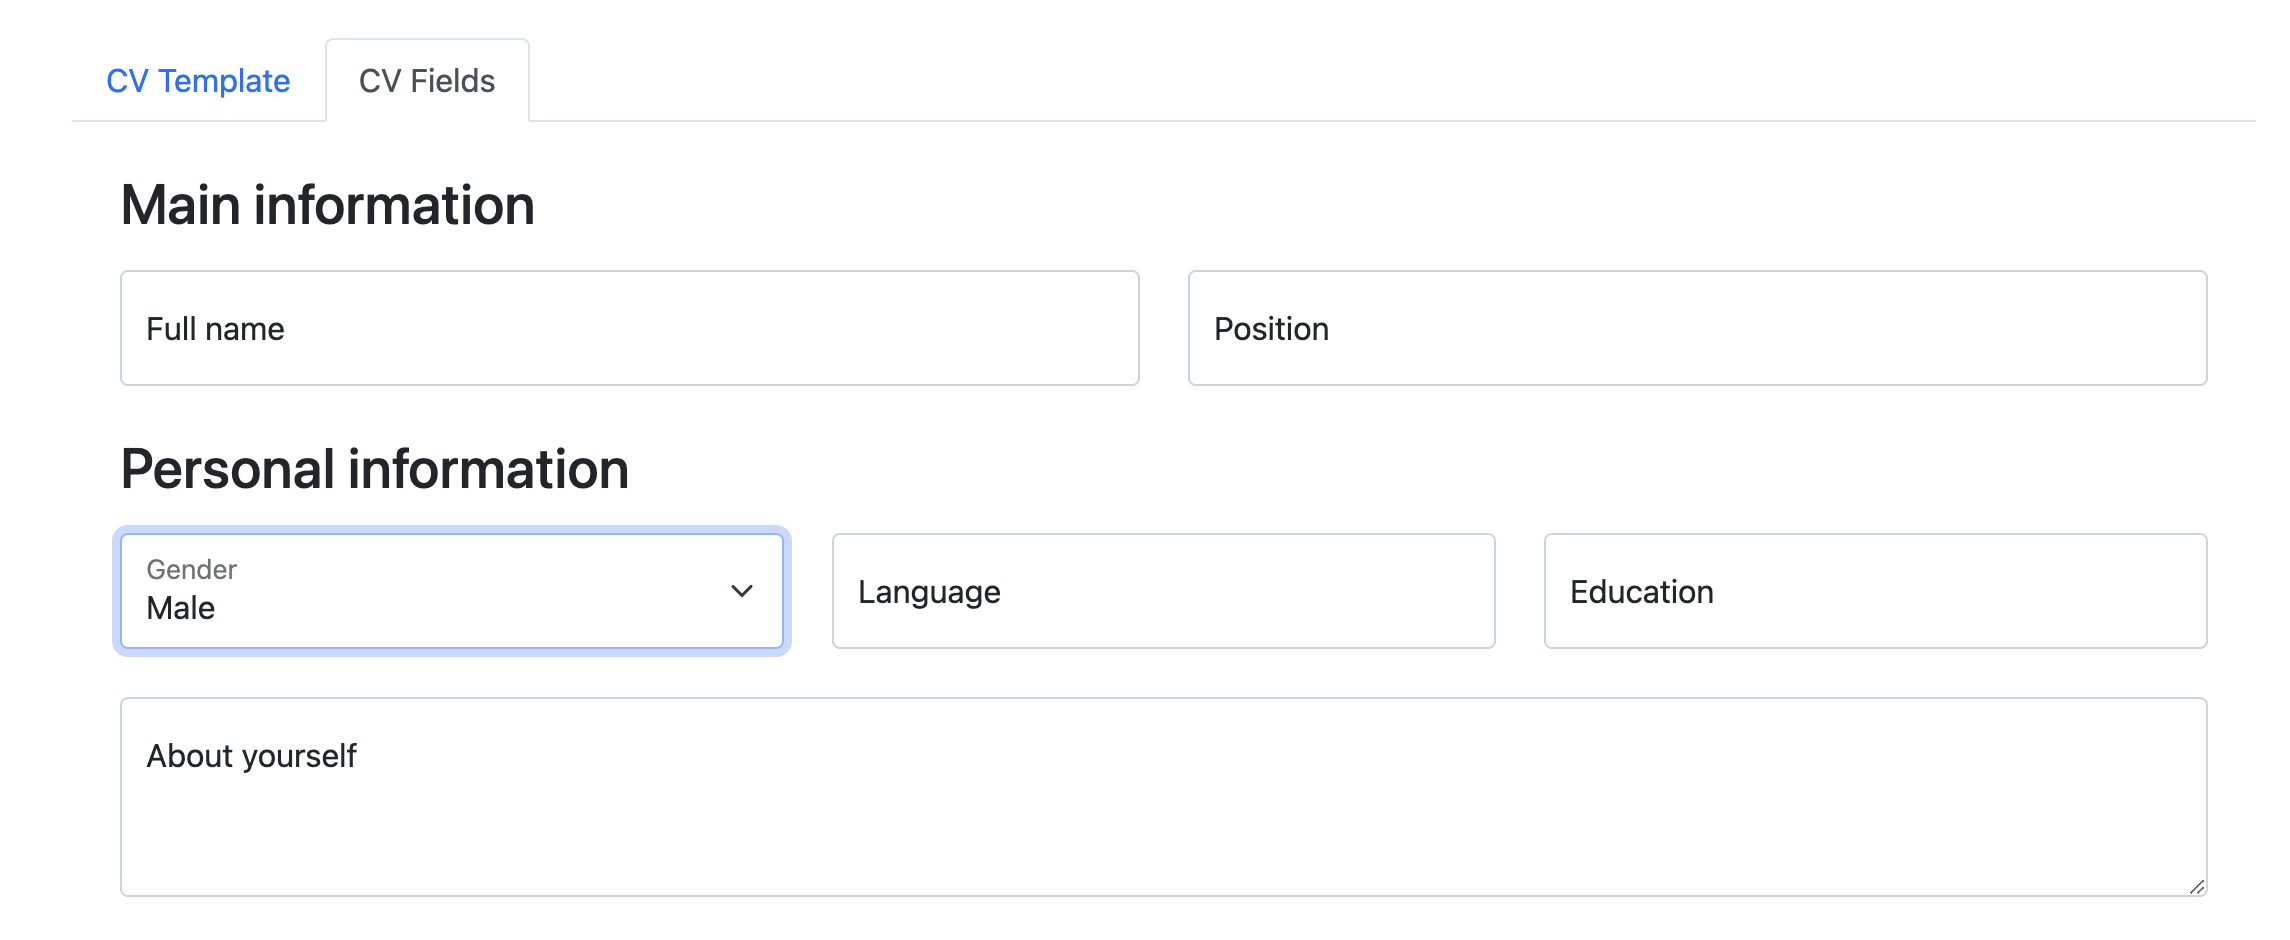
\includegraphics[width=12cm]{images/image24.png}
    \caption{\label{fig:24}%
        Отображение вкладки ввода данных}
\end{figure}


Структура хранения данных о пользователе представляет из себя json-файл, содержащий
все описанные выше поля, вроде имени, даты рождения, пола и так далее. Данный выбор
формата универсален в рамках нашего приложения и позволяет взаимодействовать с 
информацией быстрым и удобным способом.
\begin{minted}[fontsize=\small, breaklines=true, style=bw, linenos]{json}
"last_name": "Константинопольский",
"first_name": "Константин",
"middle_name": "none",
"age": 33,
"birth_date": "1991-04-30",
"gender": "male",
\end{minted}



\subsection{Реализация серверной части платформы}
После написания клиентской части приложения необходимо реализовать часть, отвечающую
за перенос резюме из сторонних проектов. Для решения поставленной задачи воспользуемся
парсером html-страницы на основе библиотеки Puppeteer. Инициируем новый проект аналогично 
тому, что было в реализации клиентской части и добавим библиотеку для скраппинга:
\begin{minted}[fontsize=\small, breaklines=true, style=bw, linenos]{bash}
mkdir parser-cv-editor
cd parser-cv-editor
npm init
yarn add puppeteer
\end{minted}


Работа парсера заключается в создании экземпляра браузера и выполнении заранее прописанных
действий. Для этого создадим файл browser.js и опишем логику работы компонента.
Так как браузер будет открываться в терминальном состоянии – его визуальное
представление необходимо только для отладки работы и во время публикации параметр 
можно выключить:
\begin{minted}[fontsize=\small, breaklines=true, style=bw, linenos]{js}
const puppeteer = require('puppeteer');
async function startBrowser(){
	let browser;
	try {
	    console.log("Opening the browser");
	    browser = await puppeteer.launch({
	        headless: true,
	        args: ["--disable-setuid-sandbox"],
	        'ignoreHTTPSErrors': true
	    });
	} catch (err) {
	    console.log("Could not create a browser instance => : ", err);
	}
	return browser;
}
module.exports = {
	startBrowser
};
\end{minted}


За управлением экземпляра браузера отвечает pageController.js. В его задачи входит
проход по указанной странице и сохранение полученных данных в хранилище в формате 
json. Для этого подключается с помощью require в Node JS подключается работа с файловой 
системой, после чего инициализируется объект браузера и через асинхронную функцию
происходит считывание страницы с её последующей записью. Дополнительно реализуем
обработчик исключений чтобы работа серверной части не нарушалась в случае возникновения
ошибок как в момент перехода на страницу, так и в момент записи информации:
\begin{minted}[fontsize=\small, breaklines=true, style=bw, linenos]{js}
const fs = require('fs');
async function scrapeAll(browserInstance){
    let browser;
	try{
	    browser = await browserInstance;
	    let scrapedData = {};
	    scrapedData = await pageScraper.scraper(browser);
	    fs.writeFile("data.json", JSON.stringify(scrapedData), 'utf8', function(err) {
		    if(err) {return console.log(err);}
		    console.log("Done");
	    });
    } catch(err){console.log("Error in ", err);}
}
module.exports = (browserInstance) => scrapeAll(browserInstance)
\end{minted}


После описания вспомогательных файлов серверной части платформы необходимо реализовать
точку входа в приложение. Для этого в index.js подключим вышеописанные компоненты,
создадим экземпляр браузера и запустим работу контроллера с данным объектом:
\begin{minted}[fontsize=\small, breaklines=true, style=bw, linenos]{js}
const browserObject = require('./browser');
const scraperController = require('./pageController');
let browserInstance = browserObject.startBrowser();
scraperController(browserInstance)
\end{minted}


\subsection{Публикация платформы единого резюме}
Перед публикацией необходимо изменить файл настроек проекта, указав
точку входа и конфигурацию скрипта в файле package.json:
\begin{minted}[fontsize=\small, breaklines=true, style=bw, linenos]{json}
"default": "index.html",
"scripts": "start": "parcel ./index.html"
\end{minted}


Так как платформа работает в режиме сервера – публикация в виде статичной страницы
не представляется возможным, поэтому воспользуемся хостингом Netlify, позволяющим 
реализовать данную потребность. Первоначально необходимо загрузить свой код в 
систему контроля версий GitHub, после чего связать аккаунт с аккаунтом хостинга,
синхронизировать репозитории и настроить параметры публикации. В итоговом виде 
платформа соберётся в оптимизированный для получения пользователем вид, 
закэшируется в папке dist и будет выдаваться браузеру при обращении по ссылке.
Настройки публикации сайта в Netlify представлены на рисунке~\ref{fig:25}.
\begin{figure}[!ht]
    \centering
    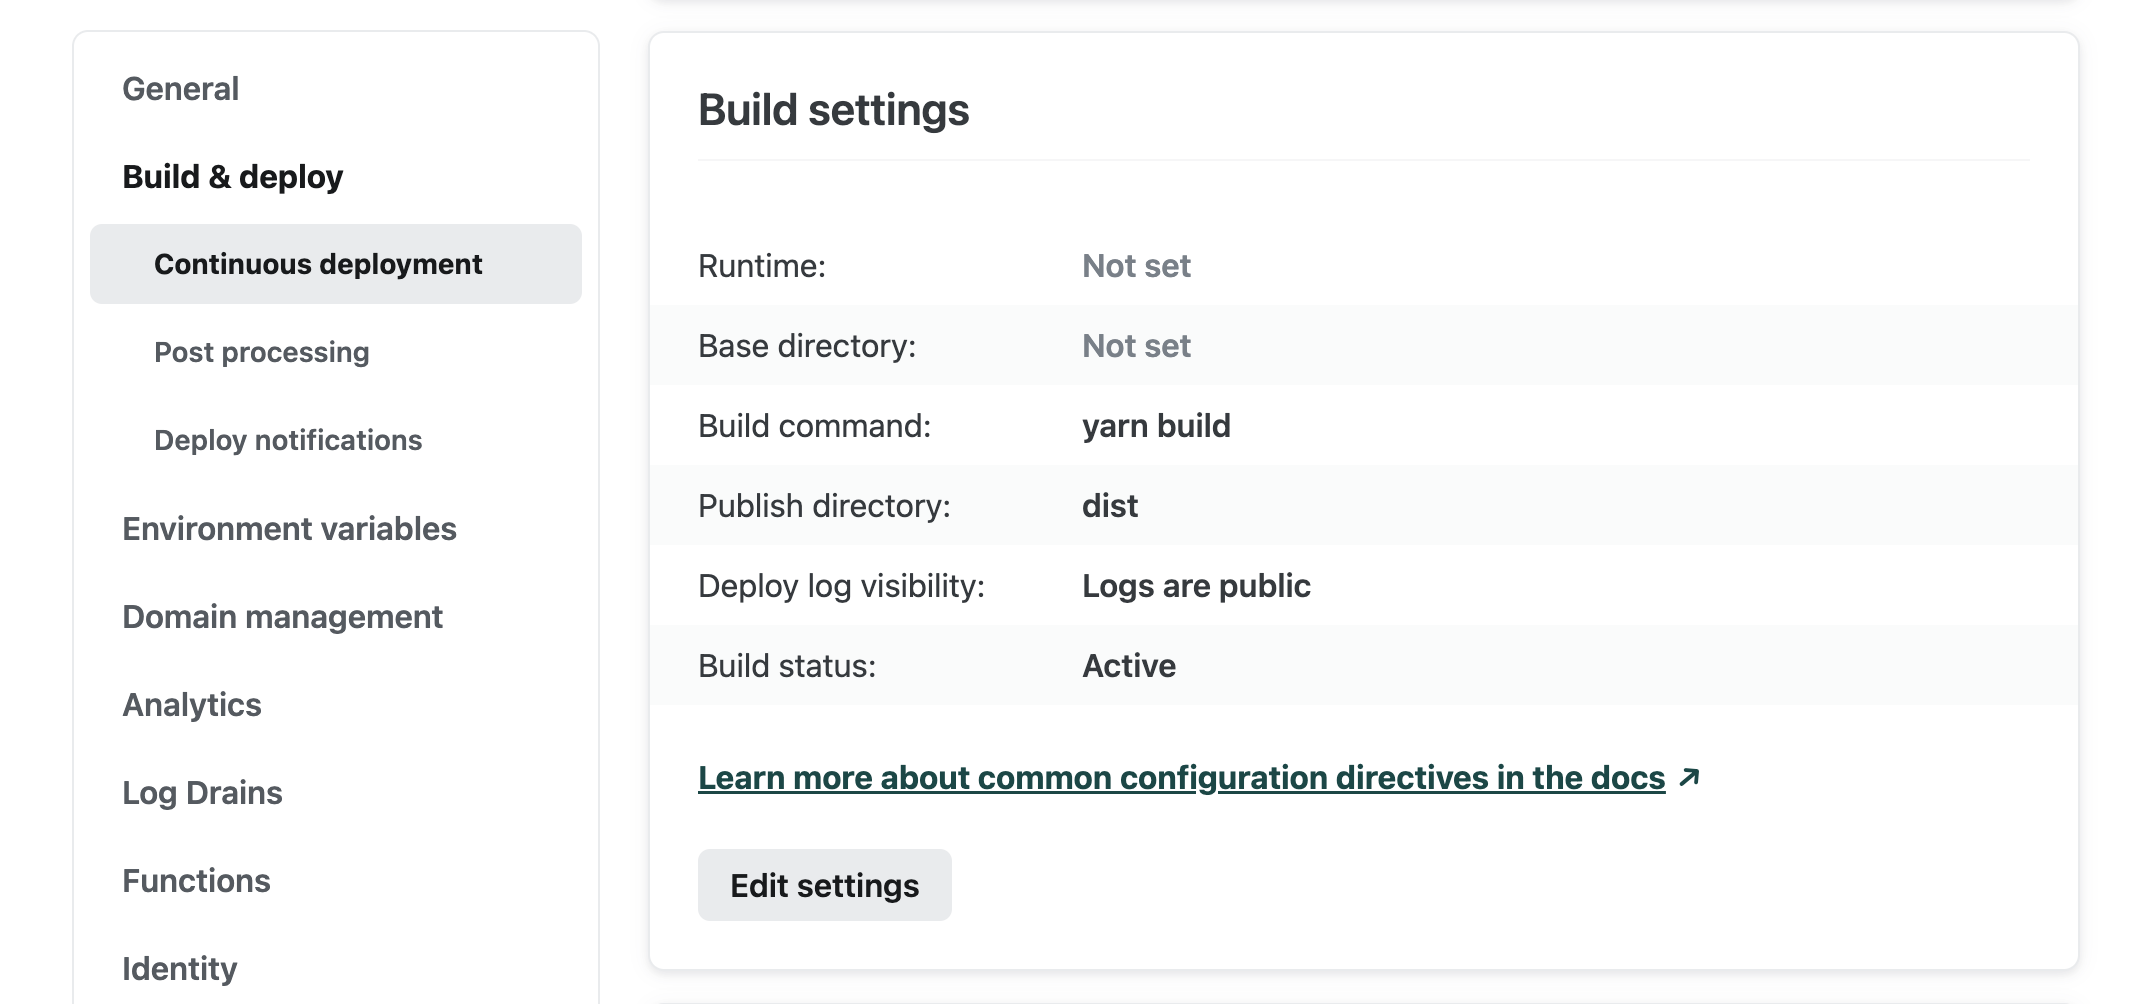
\includegraphics[width=12cm]{images/image25.png}
    \caption{\label{fig:25}%
        Настройка публикации сайта}
\end{figure} 

После реализации кода мы получили готовый сервис, в котором написаны 
все задуманные на данном этапе функции. Итоговый вид главной страницы 
проекта показан на рисунке~\ref{fig:26}.
\begin{figure}[!ht]
    \centering
    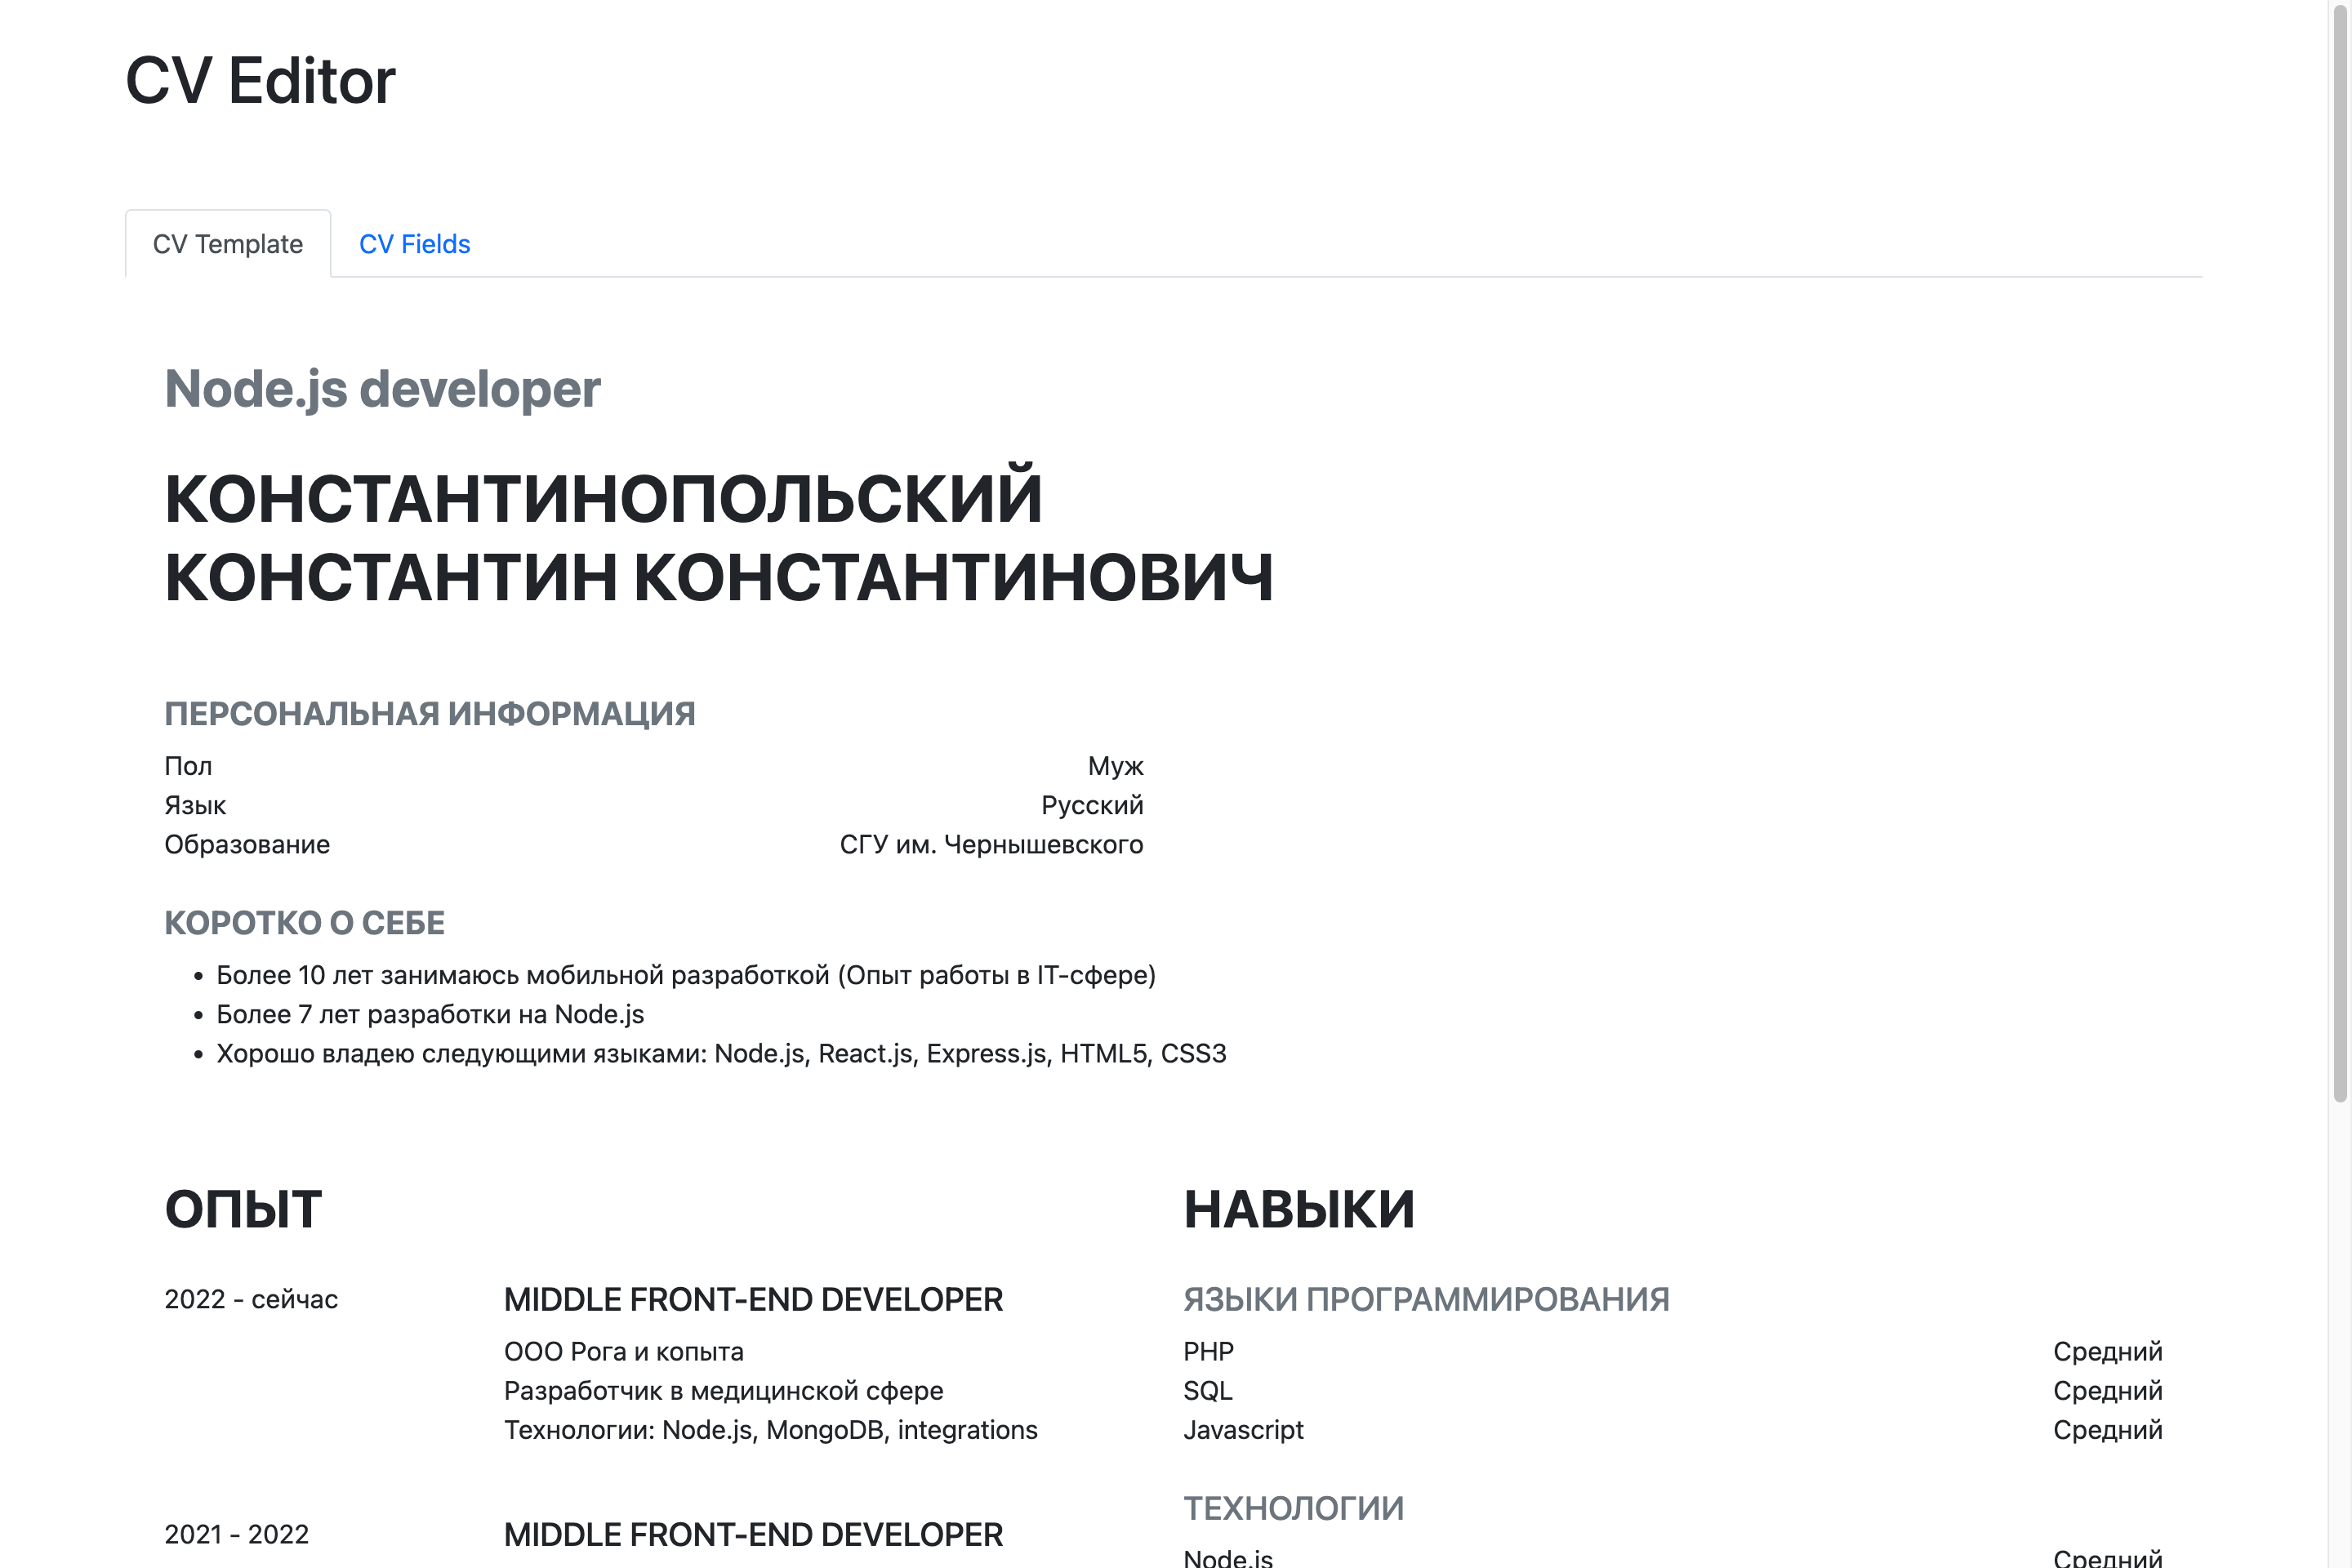
\includegraphics[width=12cm]{images/image26.png}
    \caption{\label{fig:26}%
        Итоговый вид страницы проекта}
\end{figure} 


\newpage
\conclusion
В результате проведения исследовательской работы были приобретены навыки анализа 
качества и эффективности научной литературы в области разработки сервисов 
с автоматическим обновлением данных, достигнут навык анализирования конкурентных 
платформ для создания резюме и сформулирован собственный метод разработки 
единой платформы резюме, тем самым было достигнуто полное выполнение поставленных задач.

В качестве объектов анализа научной литературы выступили статьи по темам составления 
резюме, их анализа со стороны социологии, а также статьи, в которых рассматриваются 
инструменты для веб-разработки. С учётом проведённого анализа научной литературы 
были составлены основные требования для разработки будущей платформы как с технической 
стороны, так и со стороны гуманитарно-социальных наук.

Анализ конкурентных платформ позволил выявить слабые стороны существующих сервисов, 
на основании которых был разработан функционал собственной единой платформы 
резюме, включающей в себя серверную и клиентскую части приложения с последующей
публикацией проекта на серверном хостинге для корректного взаимодействия 
с возможностями платформы.



% Библиографический список, составленный вручную, без использования BibTeX
%
% \begin{thebibliography}{99}
%   \bibitem{Ione} Источник 1.
%   \bibitem{Itwo} Источник 2
% \end{thebibliography}

% Отобразить все источники. Даже те, на которые нет ссылок.
% \nocite{*}

% Меняем inputencoding на лету, чтобы работать с библиографией в кодировке
% `cp1251', в то время как остальной документ находится в кодировке `utf8'
\inputencoding{cp1251}
\bibliographystyle{gost780uv}
\bibliography{thesis}
\inputencoding{utf8}

% При использовании biblatex вместо bibtex
% \printbibliography

% Окончание основного документа и начало приложений Каждая последующая секция
% документа будет являться приложением
\appendix

\end{document}
